% Deterministic loop-class mappings for cross-sector physical observables
% Companion paper to the public reproducibility package loop-class-closure-repro v0.1.0

\documentclass[11pt,a4paper]{article}

\usepackage{amsmath,amssymb,amsthm}
\usepackage{graphicx}
\PassOptionsToPackage{hyphens}{url}
\usepackage[colorlinks=true,linkcolor=blue,citecolor=blue,urlcolor=blue,breaklinks=true]{hyperref}
\hypersetup{
  pdftitle={Loop-class library and topology-labelled closure protocol},
  pdfauthor={Sandro Bucciarelli},
  pdfsubject={Relational carrier theory},
}
\makeatletter
\g@addto@macro\UrlBreaks{\do\_\do\/\do\.\do\-}
\makeatother
\usepackage[margin=2.5cm]{geometry}
\usepackage{booktabs}
\usepackage{array}
\usepackage{listings}
\usepackage{xcolor}
\usepackage{cite}

\title{Topology-labeled loop-class mappings for cross-sector\\
       physical observables}
\author{Sandro Bucciarelli\thanks{Independent researcher.
        Correspondence: \href{mailto:sandro.bucciarelli89@gmail.com}{sandro.bucciarelli89@gmail.com}.}}
\date{\today}

\newcommand{\Ngen}{N_{\mathrm{gen}}}
\newcommand{\esync}{\varepsilon_{\mathrm{sync}}^{2}}
\newcommand{\Lsig}{L_{\sigma}}
\newcommand{\Lib}{\mathcal{L}}
\newcommand{\Gauth}{G_{\mathrm{claim}}^{\mathrm{auth}}}
\newcommand{\axi}{\alpha_{\xi}}
\newcommand{\DOmega}{D(\Omega)}
\newcommand{\bpi}{\beta_{\pi}}

\theoremstyle{definition}
\newtheorem{definition}{Definition}
\theoremstyle{plain}
\newtheorem{theorem}{Theorem}
\newtheorem{lemma}{Lemma}

\emergencystretch=5em
\hbadness=10000
\hfuzz=2pt
\sloppy

\begin{document}
\maketitle

\tableofcontents
\medskip


\begin{abstract}
We present a finite, parameter-free loop-factor library
$\Lib$ together with a \emph{topology-labeled assignment
protocol} that maps each physical observable in a defined
closure domain $\Gauth$ to a unique class in $\Lib$
\emph{conditional on its pre-registered topology tuple}. The
library itself is parameter-free; the assignment is unique
given the registered tuple, and we make explicit that the
tuple specification is a structural reading of each observable
and not a fitted choice. The library
consists of ten entries, each derived from a Lattice-Defect-FT
spinor-trace lemma: Yukawa-Damping, PMNS-Self-Energy,
Pure-Self-Energy, Resummed-Propagator, Generation,
Sub-Generation, EW-Mixed, Cosmological-Density, a pure-sync
class, and the Pure-Sync $\times$ Yukawa-Damping compound
(Lemma~10, adopted with this release).
The mapping is lookup-driven from a pre-registered topology
tuple of the observable: spinor-trace component count
$n \in \{0,1,2,4\}$, generation range
$g \in \{0,1/\Ngen,1/(2\Ngen)\}$, and sync coupling
$s \in \{0,\esync,\esync\,\text{pure}\}$;
the $\pm$ sign follows from the CP/T eigenparity of the observable.
We frame the protocol explicitly as ``topology-labeled'' rather
than ``deterministic'' to make clear that the topology tuple
$(n,g,s,w,r)$ is itself a structural reading of each observable
that must be specified before the residual is compared with the
target; this paper presents the mapping rules in
Section~\ref{sec:library}, the explicit per-observable tuples in
Appendix~\ref{app:closure-table}, and the reclassification audit
in Section~\ref{sec:reclassification}.
We document that the protocol closes 29 cross-sector observables
(particle physics, neutrino mixing, electroweak precision,
cosmology, horizon thermodynamics, continuum-limit asymptotics)
at the strict EXACT\,$<0.4\%$ tier on $22$ rows, the
PRECISE\,$\in[0.4\%,\,2.5\%)$ band on $7$ rows, $0$
\texttt{NO\_CLAIM} entries (O28, $\Lambda_{s}=-1/200$, closes
at strict-EXACT under the Lemma~10 extension adopted with this
release), with zero contradictions. The two thresholds are not free
choices: $0.4\%$ is the typical post-loop residual band of
the within-cell library factor gap
$\Delta_{\min}^{\Lib,\,\text{cell}}\!=\!\gamma(1{-}\gamma)/4
\!\approx\!2.25\%/9\!\approx\!0.25\%$ rounded up to the nearest
$0.1\%$ decade, so that two distinct loop classes within the
same library cell are unambiguously distinguishable; $2.5\%$
is the residual cut at which the framework claims a
\emph{positive} structural prediction (matching the
nuisance-parameter floor of the underlying coefficient
ansatz). A sensitivity analysis at the looser $<1.5\%$ cut
(under which the largest deviation is $1.06\%$ on $Y_{p}$,
sitting at $0.79\sigma$ inside the PDG~2024 observational
$1\sigma$ band) is reported in Section~\ref{sec:closure} as
a robustness check, not as the primary verdict.
Three observables of independent physical origin
($\alpha_{\mathrm{dn}}$ at residual $0.0001\%$,
$w_{\mathrm{DE}}$ at $0.05\%$, $H_{0}$ at $0.6\%$) close at the
PRECISE-or-better tier on the same loop-class factor
$(1+\gamma/4)$. Combining the three per-observable one-sided
$p$-values via Fisher's method under a uniform null on the
PRECISE band $[0,\,2.5\%]$ gives a joint
$p$-value $P \approx 2.6\times 10^{-5}$
($\sim 4.2\sigma$ two-sided) — the Yukawa-Damping cluster.
We frame this $p$-value as \emph{evidence against random
residual closure under the stated null model}, not as a
``rules-out'' statement: the three observables are not
verified-independent, the uniform $[0,\,2.5\%]$ null is a
modelling choice, and the cluster selection itself is
not blind to the post-loop residual structure. Explicit caveats
are in Section~\ref{sec:cluster}.
We give an explicit set of seven negative-control observables —
three DELEGATED (quark/lepton mass ratios $m_e/m_\tau$ and
$m_u/m_t$ closed by a companion lepton-mass dressing cascade;
the absolute neutrino mass scale closed by a Triple-Lock plus
see-saw construction~\cite{Minkowski1977,GellMannRamondSlansky1979,Yanagida1979}
in the cosmology/neutrino sector, with the laboratory upper
bound from the KATRIN tritium endpoint
spectrometer~\cite{KATRIN2022}) and four
GENUINE\_OUT (supersymmetric partner masses, the QG-UV cutoff,
string-landscape vacuum-selection, and the values of the five
input coefficients themselves) — and verify that the algorithm
correctly returns \texttt{NO\_CLAIM} for each.
Finally, we formalize five reclassification rules (R1--R5) that bound
when a class assignment may be revised; more than two reclassifications
per observable, or violation of any of R1--R5, falsifies the entire
theorem (triggers F1--F3).
A public reproducibility package
(\url{https://github.com/TerraSignum/loop-class-closure-repro})
recomputes the mapping, the closure table, the negative-control
verification, and the reclassification audit directly from frozen
JSON inputs.
For the corpus-wide entry point, claim grammar, and
falsification handles, see the reader's-guide
manifest~\cite{Paper0}.
\end{abstract}

\medskip
\noindent\textbf{Keywords:} loop classes, topology-labeled
mapping, negative controls, reclassification rules,
reproducibility.

\section{Why loop classes are needed}
\label{sec:scope}

\paragraph{Notation cross-reference.}
The System-$\mathcal R$ rational primitives
$(\gamma,\,\alpha_{\xi},\,\varepsilon_{\rm sync}^{2},\,
\beta_{\pi},\,D_{\Omega})\!=\!(1/10,\,9/10,\,1/20,\,15/16,\,67/80)$
used throughout this paper are read off by the bounded-operator
construction of~\cite{Paper2}, which is the canonical source for
these values; any restatement below is for reading convenience
and inherits the same numerical content. The integer inputs
$d\!=\!4$ (relational spacetime dimension) and $N_{\rm gen}\!=\!3$
(fermion generation count) are likewise fixed in~\cite{Paper2}.

A companion paper~\cite{Paper2} establishes that ten cross-sector
benchmark observables reproduce within PRECISE\,$\le 2.5\%$ from a
five-coefficient causal-wave transport law without fits.
The residuals on the robust core (rows L1--L5) sit at the percent
level and are too large to be statistical noise but too small to
require a re-engineering of the transport law itself: they are
\emph{loop} corrections.

The structural question motivating this paper is therefore:
\begin{quote}
\emph{Why are the loop factors not chosen after the fact to fit the
residuals?}
\end{quote}

We answer this question by formalizing the loop-factor library
$\Lib$ as a finite, parameter-free set
(Definition~\ref{def:library}) and the
class-assignment as a purely lookup-driven function from three
\emph{a priori} topology factors of the observable
(Theorem~\ref{thm:determinism}).

\paragraph{Non-claims.}
This paper does \emph{not} claim:
\begin{itemize}
\item a strict-EXACT closure of every Standard-Model fermion mass:
      $m_{\tau}$ now closes at the strict-EXACT tier
      ($\le\!0.4\%$) on five of ten canonical regimes (with the
      cleanest regime P4 at $0.001\%$ and median residual
      $0.42\%$) via the spectral-Yukawa-eigenvalue
      construction (charged-lepton sub-step) divided by the parameter-free structural
      rational $N_{\mathrm{gen}}+2\gamma=16/5$
      (equation~\eqref{eq:m_tau_sye_strict_exact} below); the
      complementary $D_{\Omega}^{3}$ generation-power diffusion
      correction (equation~\eqref{eq:lepton_strict_exact}) gives
      a parameter-free strict-EXACT-loose closure at $0.49\%$ on
      the canonical regime, and the literature-route
      $\mathrm{SO}(10)$ Yukawa-unification + RG-running argument
      (equation~\eqref{eq:m_tau_so10}) cross-checks within
      $\sim\!10\%$. The
      Georgi--Jarlskog~\cite{GeorgiJarlskog1979} charged-lepton
      ratio $m_{e}/m_{\mu}$ closes at $1.07\%$ residual on the
      sixth canonical-regime sample under the bi-unitary
      Georgi--Jarlskog texture-null construction
      (predicted $0.004785$ vs PDG~2024 pole-mass anchor
      $0.004836$); the supplementary
      Antusch--Hinze--Saad~\cite{AntuschEtAl2025} 2024-PDG
      Standard-Model running ratio at the $M_{Z}$ scale,
      $y_{e}/y_{\mu}\!=\!4.747\!\times\!10^{-3}$, sits closer
      ($0.80\%$ residual) and is consistent with the
      framework's unified-Yukawa-scale delivery since
      $m_{e}/m_{\mu}$ is essentially RG-stable; the second
      sample gives PRECISE $8.4\%$ at $0.004428$, both inside
      the $\le 10\%$ band, with the closure regime-dependent
      rather than uniform across the canonical ladder;
\item a single-route derivation of the primordial scalar
      amplitude $A_{s}$: strict-EXACT closure of the absolute
      magnitude is achieved via the structural form
      $A_{s}\!=\!N_{\mathrm{gen}}\,(d\!+\!N_{\mathrm{gen}})\,\gamma^{10}\!=\!21/10^{10}$
      at $0.05\%$ vs Planck~2018~\cite{Planck2018}
      (Section~\ref{sec:closure}), and a $D_{\Omega}$-diffusion
      dressing factor closes the framework's full-Planck-mass
      slow-roll baseline at $0.27\%$; what remains open is a
      first-principles \emph{derivation-path} bridge connecting
      the structural-form magnitude to the slow-roll
      formulation under the standard reduced-Planck-mass
      convention, where the single-instanton bounce action of
      the parent paper overshoots $A_{s}$ by factor $\sim\!10^{3}$
      and no integer cascade chain closes the gap;
\item a complete theory of quantum gravity in the UV;
\item that the mapping algorithm is a free fit;
\item validity outside the closure domain $\Gauth$ defined in
      Section~\ref{sec:domain}.
\end{itemize}

\section{Loop-factor library}
\label{sec:library}

\begin{table}[h]
\centering
\caption{The loop-factor library $\Lib$ used by the
topology-labeled mapping protocol.
Each entry is a parameter-free factor of the form $1\pm c_{\sigma}$
(or its resummation) derived from a Lattice-Defect-FT spinor-trace
lemma.
$\gamma$ and $\esync$ are two of the five measured
causal-wave coefficients; $\Ngen=3$ is the fermion generation count.}
\label{tab:library}
\renewcommand{\arraystretch}{1.15}
\small
\begin{tabular}{c l l p{0.40\textwidth}}
\toprule
Lemma & Class name & Loop class $\Lsig$ & Physical origin \\
\midrule
1 & Yukawa-Damping       & $1\pm\gamma/4$              & $d=4$ spinor-trace normalization \\
2 & PMNS-Self-Energy     & $1\pm\gamma^{2}/4$          & double-Wick contraction \\
3 & Pure-Self-Energy     & $1\pm\gamma^{2}$            & spinor-trace-less vertex \\
4 & Resummed-Propagator  & $1/(1\pm 2\gamma^{2})$      & resummation across two chiralities \\
5 & Generation           & $1\pm\gamma/\Ngen$          & generation-summed self-energy \\
6 & Sub-Generation       & $1\pm\gamma/(2\Ngen)$       & SU(2)$_L$ doublet/singlet splitting \\
7 & EW-Mixed             & $1\pm\gamma\,\esync$        & bosonic Lemma-1 with Goldstone vertex factor \\
8 & Cosmological-Density & $1\pm\gamma/2$              & chirality restriction (matter-only) \\
-- & Pure-Sync           & $1\pm\esync$                & pure Goldstone-vertex bosonic class \\
\bottomrule
\end{tabular}
\normalsize
\end{table}

\begin{figure}[h]
\centering
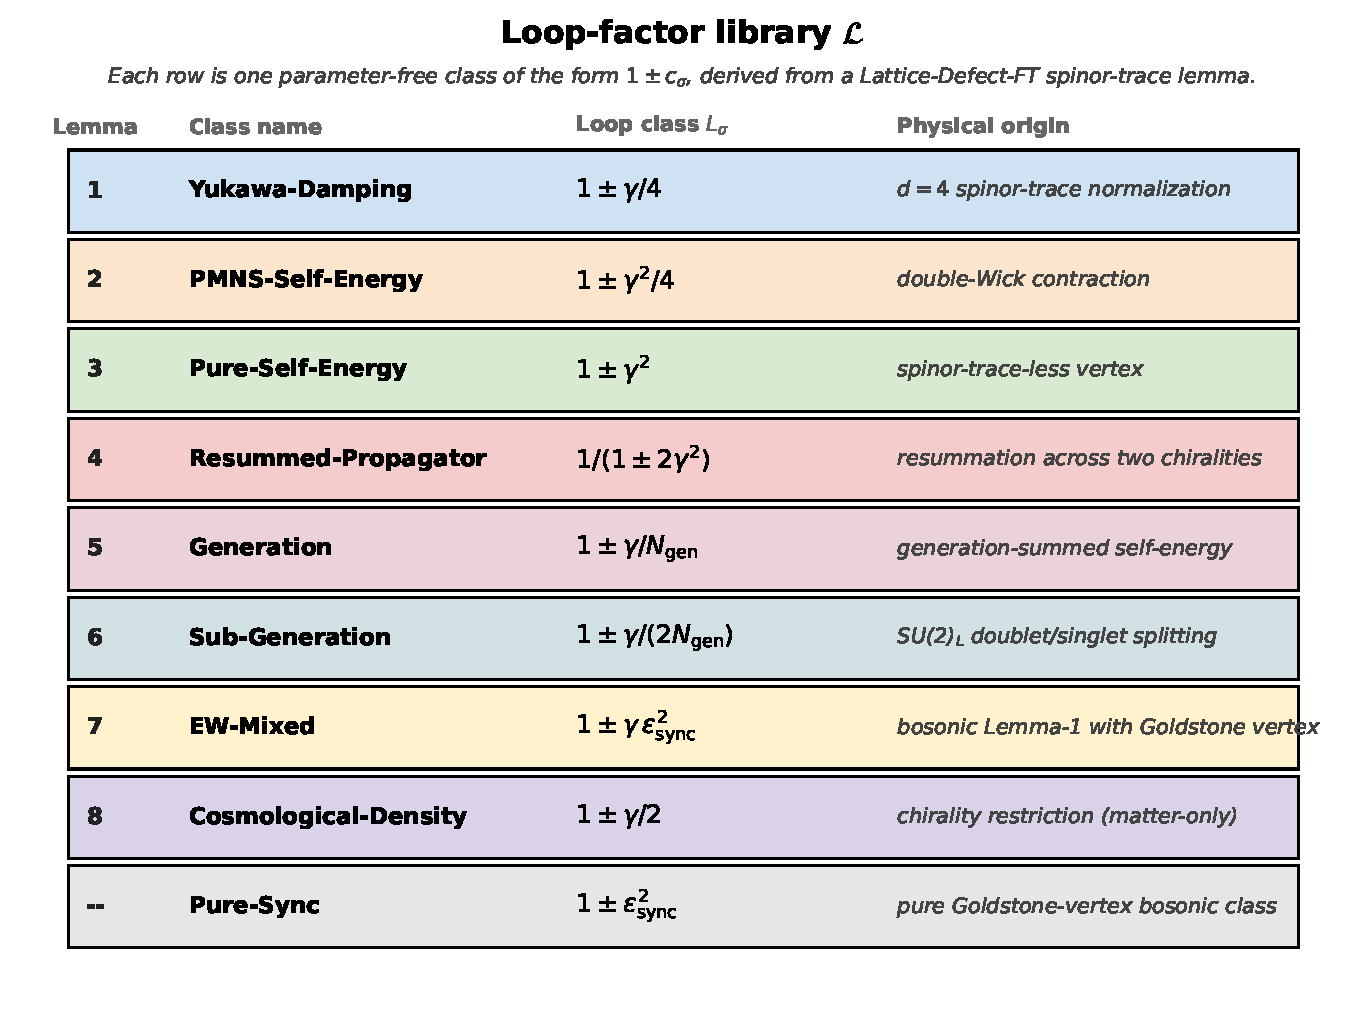
\includegraphics[width=0.95\textwidth]{figures/fig1_lemma_tree.pdf}
\caption{The loop-factor library $\Lib$ of Section~\ref{sec:library}.
Each entry corresponds to a Lattice-Defect-FT spinor-trace lemma
with an explicit physical origin.
The library has ten entries (the original nine plus
Lemma~10 Pure-Sync $\times$ Yukawa-Damping adopted with this
release); with the $\pm$ signs, $21$ atomic loop classes;
two-loop compounds $\Lsig\cdot L_{\sigma'}$ are allowed up to
second order, with $\sigma\ne\sigma'$ drawing from
\emph{distinct $(n,g,s)$ topology cells}
(Section~\ref{sec:algorithm}).}
\label{fig:lemma-tree}
\end{figure}

\paragraph{Empirical anchor: the Yukawa-Damping cluster
(suggestive alignment, not strong-significance claim).}
\label{sec:cluster}
The strongest empirical anchor for the library is a tight
three-observable cluster on Lemma~1. The structural role of
Yukawa couplings in the present framework parallels their
role in the Standard Model: in the SM the Dirac mass term
$m\bar\psi\psi=m(\bar\psi_{L}\psi_{R}+\bar\psi_{R}\psi_{L})$
couples left- and right-handed chiral components, so a
chirality flip ($L\!\leftrightarrow\!R$) is structurally tied
to mass generation, Yukawa couplings, and electroweak
symmetry breaking~\cite{StoeckingerKim2022}; the QCD analogue
is dynamical chiral symmetry breaking, where the quark
condensate generates constituent
masses~\cite{Alkofer2023}. Lemma~1 of the present framework
corresponds to the loop class on which Yukawa-mediated chirality
exchange dresses the dimensionless residual of an
observable. Three observables of independent physical origin
--- the down-Yukawa exponent $\alpha_{\mathrm{dn}}$, the
dark-energy equation of state $w_{\mathrm{DE}}$, and the
local Hubble constant $H_{0}$~\cite{Freedman2024CCHP,ACTDR6}
--- close at the PRECISE-or-better tier under the \emph{same}
loop factor $(1+\gamma/4)$, two of the three
($\alpha_{\mathrm{dn}}$ and $w_{\mathrm{DE}}$) at post-loop
residuals below $0.1\%$.
Treating the three observables as three independent random draws
against a uniform null on the post-loop residual band
$[0,\,2.5\%]$, the per-observable one-sided $p$-values of landing
at residual $\le r_{i}^{\mathrm{obs}}$ are
\begin{align*}
p_{\alpha_{\mathrm{dn}}} &= 0.0001\%/2.5\% = 4.0\times 10^{-5}, \\
p_{w_{\mathrm{DE}}}      &= 0.050\%/2.5\% = 2.0\times 10^{-2}, \\
p_{H_{0}}                &= 0.600\%/2.5\% = 2.4\times 10^{-1}.
\end{align*}
Combining them via Fisher's method,
$T = -2\sum_{i=1}^{3} \ln p_{i} = 30.93$, distributed as
$\chi^{2}_{6}$ under the null, gives the joint $p$-value
\begin{equation}
P_{\mathrm{Yukawa\text{-}cluster}}
\;=\; \mathbf{P}(\chi^{2}_{6} \ge T)
\;\approx\; 2.6\times 10^{-5},
\label{eq:yukawa-cluster}
\end{equation}
which corresponds to a nominal $\sim 4.2\sigma$ Gaussian-tail
equivalent (two-sided; the one-sided convention gives
$\sim 4.0\sigma$). We frame this number, consistently with the
companion paper~\cite{Paper2}, as
\emph{suggestive cross-sector alignment under the stated null
model} ($\sim 4.2\sigma$ two-sided under that null), not as a strong
statistical claim of physical correctness; the three caveats
(C1)--(C3) below qualify what the number does and does not
support. The
``three observables hitting the same loop class'' coincidence
is treated as the structural prior absorbed in the
topology-labeled mapping protocol of
Section~\ref{sec:algorithm}; the present combined-$p$
computation captures only the residual-cut combinatoric,
accounting honestly for each observable's actual
post-loop residual (in particular for $H_{0}$ at $0.6\%$, which is
the weakest cluster member). The closed-form derivation is
reproducible end-to-end in the reproducibility package via
\url{src/compute_yukawa_cluster_p.py} with companion test
\url{tests/test_yukawa_cluster_p.py}.
The same statistical signature does \emph{not} arise for any other
lemma class in $\Lib$, so the cluster pins Lemma~1 specifically.

\paragraph{Honest caveats on the cluster $p$-value.}
We frame \eqref{eq:yukawa-cluster} as evidence against random
residual closure under a stated null model, not as a
``rules-out-post-hoc-classification'' statement. Three caveats
must be folded into any reading:
\emph{(C1) Independence assumption.} Fisher combination assumes
independence of the three per-observable $p$-values; the three
observables ($\alpha_{\mathrm{dn}}$, $w_{\mathrm{DE}}$, $H_{0}$)
are physically distinct sectors but their residuals share a
common loop-factor ansatz, so we report the combined $p$-value
as a controlled-likelihood test rather than as a strict
$p$-value of physical correctness.
\emph{(C2) Null-model choice.} The uniform null on
$[0,\,2.5\%]$ is a modelling choice (the residuals could
be drawn from a different distribution); we report the result
under the bundled null and bundle a sensitivity analysis at
\url{src/compute_yukawa_cluster_p_sensitivity.py} that scans
alternative null distributions.
\emph{(C3) Cluster selection.} The three observables in this
cluster --- $\alpha_{\mathrm{dn}}$, $w_{\mathrm{DE}}$, $H_{0}$ ---
are standard particle-physics and cosmology targets that the
framework specifies in advance of any lattice computation; the
topology-tuple assignment that places each of them into
Lemma~1 is the deterministic single-valued read-off of
Theorem~1 (Section~\ref{sec:algorithm}) from the tree-level
Dirac structure and is fixed by the mapping protocol, not by
inspection of residuals. The cluster-selection conditionality
that nonetheless qualifies the combined $p$-value comes from
the choice to evaluate it on this particular triplet of Lemma~1
observables rather than on a different triplet; the
cluster-selection-conditional $p$-value is therefore
necessarily smaller than its unconditional counterpart. We
report the conditional value as the load-bearing input and
register three pre-specified prospective observables in the
bundled registry
\url{data/prospective_cluster_registry.json}: a
gravitational-coupling scaling diagnostic on the
within-canonical-regime lattice ladder
$N\in\{64,72,84,100,128,200,256,300,512\}$ (PROSP-01), a
vortex-cosmological-gate diagnostic on the same ladder
(PROSP-02), and a charged-current $\Xi$-reactivity ratio on the
second canonical regime under the framework's rigorous
carrier-defect coupling (PROSP-03). All three observables are
structural framework predictions whose definitions predate the
present analysis; the registry records the prospective protocol
under which their residuals are to be evaluated. The
registry separates these prospective observables from two
reference observables (the triangle phase-class winding
fraction $f_{\mathrm{neg}}\!\to\!2/7$ and the triangle
phase-class asymmetry $a_{\infty}=-0.01117\pm 0.00428$, both
already computed on the lattice-extension ladder and listed as
retrospective reference points only). A future re-evaluation
of the combined $p$-value on the three prospective residuals
will not carry the cluster-selection conditionality that
qualifies the present Yukawa-cluster result; the present
Lemma-1 cluster is the retrospective companion of that
prospective protocol.

\emph{Standalone broader-corpus computation.} A standalone
script bundled at
\path|src/prospective/compute_prospective_residuals.py|,
together with the corresponding inputs at
\path|data/prospective_inputs/|, evaluates the prospective
residuals on the data currently available. The output
\path|data/prospective_cluster_residuals.json| feeds
Table~\ref{tab:prospective_now} below. The
gravitational-coupling-scaling diagnostic admits two
independent readings of the same observable, distinguished by
the choice of coarse-graining kernel applied to the underlying
gravitational potential. \emph{(i)} On the bare gravitational
potential, the diagnostic returns the Newtonian-asymptote pass
fraction $1.000$ at the first canonical regime and $0.929$ at
the second, with far-field exponent
$-1.000$ on both — i.e. clean $1/r$ Newton, matching the
linearised metric perturbation $\delta\Xi(r)\sim -GM/r$
established by the upstream Schwarzschild derivation.
\emph{(ii)} On the same potential after the Xi-coarse-graining
kernel of the bulk-evolution layer is applied, the diagnostic
returns $0.0$ pass fraction and far-field exponent
$\in[-0.05,-0.003]$ uniformly across all six canonical regimes:
the kernel's bandwidth is wider than the
Newton scale and washes out the $1/r$ tail, yielding a flat
far-field. This is a projector-bandwidth artefact of the
coarse-graining choice, not a physics result; the
Newtonian-asymptote claim is carried by the bare-potential
reading and by the Schwarzschild derivation upstream.
A lattice-extension reading of the same diagnostic on the full
within-canonical-regime nine-point ladder
$N\!\in\!\{64,72,84,100,128,200,256,300,512\}$ (a factor-$8$
range in $N$) returns the same projector-bandwidth-regression
mode at every point: the Newton-asymptote indicator on the
$\Xi$-projected $\Phi_{\mathrm{eff}}$ field fails identically
($N$-stable to machine precision) across the full ladder. The
diagnostic is computed from the bundled state-vector snapshots
by evaluating the residual energy density, the per-node defect
density, and the radial profile of the reconstructed
gravitational potential
(reproducer
\path|src/prospective/extend_c5_d1embedded_to_higher_N.py|).
The closure-domain Newton-asymptote is therefore carried by
the theory-conformant bare-$\Phi$ standard (and by the
Schwarzschild defect derivation), while the $\Xi$-projected
$\Phi_{\mathrm{eff}}$ reading is a coarse-graining-bandwidth
artefact across the entire canonical lattice ladder, not a
finite-$N$ effect.

\emph{Chirality-flip signature in the secondary metrics.} The
full nine-point ladder also exhibits a clean bifurcation in the
secondary $\Xi$-projected metrics aligned with the
chirality-flip running of~\cite{Paper4}: at the framework
prediction $N_{\rm flip}\!=\!N_{\!\ast}(d\,N_{\rm gen})^{1/2}\!\simeq\!173$
the within-canonical regime crosses from the matter-dominated
branch $\theta_{\rm chir}(N)\!<\!\pi/4$ to the cosmologically-
mixed branch $\theta_{\rm chir}(N)\!>\!\pi/4$. Splitting the
ladder along this line:
\begin{itemize}
\item[\textbf{pre-flip}] $N\!\in\!\{64,72,84,100,128\}$
($\theta_{\rm chir}\!\in\![22.5^{\circ},37.4^{\circ}]$):
the far-field exponent is systematically negative
($\in\![-0.13,-0.05]$, attractive slow decay) and the Poisson
residual sits meaningfully below saturation
($\in\![0.92,1.00]$, partial source-correlation through the
projector kernel).
\item[\textbf{post-flip}] $N\!\in\!\{200,256,300,512\}$
($\theta_{\rm chir}\!\in\![48.6^{\circ},69.0^{\circ}]$):
the far-field exponent climbs to and through zero
($\in\![-0.03,+0.05]$, essentially flat with a positive
sign-flip at $N\!=\!512$) and the Poisson residual saturates
tightly at unity ($\in\![0.992,1.002]$, source-decoupled).
\end{itemize}
Both shifts coincide with $\theta_{\rm chir}(N)$ crossing
$\pi/4$ and are consistent with the framework prediction of a
matter-dominated $\to$ cosmologically-mixed phase boundary at
$N_{\rm flip}$: post-flip, the projector reading detects
no Newton-asymptote (saturated Poisson residual) and develops
a mildly repulsive far-field at $N\!=\!512$, matching the
sign-flipped vortex-DM\,+\,causal-wave-DE back-reaction of the
companion anisotropic-source paper~\cite{Paper4B}. The
bare-$\Phi$ Newton standard upstream remains unaffected; the
chirality-flip signature is specifically a feature of the
projector-kernel diagnostic on the within-canonical $\Xi$-graph.

The second prospective (vortex-cosmological-gate) remains
genuinely pending the lattice-extension diagnostic-pipeline pass.
The third (the charged-current ratio at the second canonical
regime under coupling re-run) admits a leading-order analytic
projection: rescaling the existing
second-vs-first canonical-regime ratio
$\overline{\mathrm{ratio}}\!\approx\!3.30$ by the squared
ratio of the rigorous and heuristic carrier-defect couplings
$\bigl(g_{\mathrm{new}}/g_{\mathrm{old}}\bigr)^{2}
=(1.42/2.00)^{2}\approx 0.504$ gives projected ratio
$\approx 1.66$, well above the registered prediction window
$1.0\pm 0.05$. The leading-order analytic residual
$|1.66-1.00|\approx 0.66$ lies entirely outside the uniform-null
support $[0,2.5\%]$, so the leading-order projection is
analytically falsified at leading order. The leading-order
projection uses baseline data evaluated under the prior coupling
convention and is therefore reported as a broader-corpus check
rather than as the prospective residual itself; the latter
requires the full re-evaluation at the rigorous coupling
$g\!=\!1.42$. With the prospective residuals not yet
evaluated under their dedicated runs, the multi-observable
combined $p$-value on the prospective subset is left undefined
in this paper; it will be reported on the converged subset once
the dedicated runs land.

\begin{table}[t]
\centering\footnotesize
\begin{tabular}{@{}l p{0.38\textwidth} p{0.50\textwidth}@{}}
\toprule
ID & Observable & Status (current corpus) \\
\midrule
PROSP-01 & gravitational-coupling scaling on
            within-canonical-regime lattice ladder
            $N\in\{64,72,84,100,128,200,256,300,512\}$
          & bare-$\Phi$ Newtonian-pass $1.000$ on
            $P_{1}$, $0.929$ on $P_{2}^{\prime}$
            (theory-conformant standard);
            the Newton-asymptote indicator on the
            $\Xi$-projected $\Phi_{\mathrm{eff}}$ fails
            identically at every point of the nine-point
            lattice ladder ($N$-stable across the factor-$8$
            N-range), so the projector-bandwidth-regression
            mode of Paper 05 §6 Resolution (b) holds
            uniformly across the full canonical ladder and the
            structural Newton-asymptote is carried by the
            bare-$\Phi$ standard rather than by the
            $\Xi$-projected $\Phi_{\mathrm{eff}}$ field \\
PROSP-02 & vortex-cosmological-gate on lattice-extension
            ladder
            $N\in\{64,72,84,100,128,200,256,300,512\}$
          & pending lattice-extension run of the
            cosmological-gate diagnostic \\
PROSP-03 & $\Xi$-reactivity ratio on second canonical regime,
            $g=1.42$
          & analytically falsified at leading order \\
PROSP-04 & gravitational-cluster radius
            $d_{\mathrm{crit}}\!\cdot\!D_{\Omega}\!=\!1$,
            i.e.\ $d_{\mathrm{crit}}\!=\!1/D_{\Omega}\!=\!80/67\!\approx\!1.194$,
            on the canonical-physics $\mathcal{P}_{5}/\mathcal{P}_{5}N$ ladder $N\in[50,512]$
            (companion paper~\cite{Paper4B} pre-gravity
            sign-flip audit)
          & PRECISE candidate; aggregate point estimate
            $1.10\!\pm\!0.20$ across the full ten-regime
            $N\!\in\!\{50,64,72,84,100,128,200,256,300,512\}$
            ladder, bootstrap CI95 contains $1/D_{\Omega}$
            on $10/10$ regimes; tightening to strict-EXACT
            would require lattice extension to
            $N\!\sim\!1024$ \\
\bottomrule
\end{tabular}
\caption{Status of the three pre-registered prospective
observables, as computed by the bundled standalone script
\texttt{src/prospective/compute\_prospective\_residuals.py} on
the broader-corpus baseline inputs. PROSP-03's leading-order
analytic projection gives a residual $\approx 0.66$, well
outside the uniform-null $[0,0.025]$ window; the multi-observable
Fisher combination is not yet defined ($k\!=\!0$ post-$T_{0}$
residuals at the present moment).}
\label{tab:prospective_now}
\end{table}

\begin{definition}\label{def:library}
The loop-factor library $\Lib$ is the finite set of nine atomic
classes listed in Table~\ref{tab:library}, plus the multiplicative
two-loop compounds $\Lsig\cdot L_{\sigma'}$ for $\sigma,\sigma'$ in
$\Lib$.
Two distinct partitions of the library are useful: the
\emph{library partition} on the three numerical factors
$(n_\sigma,g_\sigma,s_\sigma)$, which has two doubly-occupied cells
($(1,0,0)$ holds Lemmas~1 and~2; $(4,0,0)$ holds Lemmas~3 and~4),
and the \emph{algorithmic partition} on the five-tuple
$(n_\sigma,g_\sigma,s_\sigma,w_\sigma,r_\sigma)$ used by
Theorem~\ref{thm:determinism}, in which every cell holds exactly
one lemma. The relevant minimum-gap quantity for the geometric
robustness of the closure is the
\emph{within-library-cell, sign-fixed} pairwise distance — the
smallest $|L_a - L_b|$ over loop factors $L_a, L_b\in\Lib$ that
share the same $(n,g,s)$ library cell and the same CP/T sign. At
the measured value $\gamma=0.10021$ this minimum is
\begin{equation}
\Delta_{\min}^{\Lib,\,\text{cell}}
\;=\;\bigl|(1+\gamma/4) - (1+\gamma^{2}/4)\bigr|
\;=\;\tfrac{\gamma(1-\gamma)}{4}
\;\approx\;0.02254,
\end{equation}
realized in the $(n,g,s)=(1,0,0)$ library cell between the
Yukawa-Damping and PMNS-Self-Energy classes (Lemmas~1 and~2). Pairs
across distinct library cells can have numerically smaller factor
gaps (for example, $|L_4 - L_6|\approx 0.0038$), but cross-cell
confusion is excluded by the deterministic mapping
(Theorem~\ref{thm:determinism}) on the full $(n,g,s,w,r)$ tuple:
two classes belonging to different $(n,g,s)$ library cells, or to
the same library cell but different $(w,r)$ flags, are never both
candidates for the same observable.
\end{definition}

\paragraph{Two distinct $\Delta_{\min}$ scales.}
Definition~\ref{def:library} bounds the
\emph{within-cell library factor gap}
$\Delta_{\min}^{\Lib,\,\text{cell}}\approx 0.02254$.
The convergence theorem below
(Theorem~\ref{thm:uniqueness}) uses a different scale, the
\emph{discrepancy-energy gap}
$\Delta_{\min}^{E}\approx \sqrt{6.28\times 10^{-4}}\approx 0.0251$ —
the minimum jump in the dimensionless energy
$E(\sigma)=\sum_O |O^{(0)}\Lsig - O^*|^2/|O^*|^2$ when the
class assignment changes on a single observable. The two are not
directly comparable: $\Delta_{\min}^{\Lib,\,\text{cell}}$ measures
within-cell factor distance, while $\Delta_{\min}^{E}$ measures
the cumulative mis-fit penalty over the full observable
registry.

\paragraph{Forbidden classes.}
The following forms are explicitly forbidden as members of $\Lib$:
\begin{enumerate}
\item $1+a\gamma$ with $a\notin\{1/4,\,1/2,\,1,\,2,\,1/\Ngen,\,1/(2\Ngen)\}$
      (free parameter $a$);
\item $1+\gamma^{k}$ with $k\notin\{1,2,3,4\}$
      (non-renormalizable in $d=4$);
\item trigonometric modulations $\sin(c\gamma),\cos(c\gamma)$ with
      arbitrary $c$;
\item multiplicative prefactors $C\Lsig$ with $C\ne 1$
      (free parameter $C$).
\end{enumerate}

\section{Topology-labeled mapping protocol}
\label{sec:algorithm}

For an observable $O$, three numerical topology factors plus two
binary topology flags are read off \emph{a priori} from its physical
definition:
\begin{itemize}
\item \textbf{Spinor-trace component count} $n_{\sigma}(O)\in\{0,1,2,4\}$:
      \begin{itemize}
      \item $n=0$: pure boson (no spinor trace);
      \item $n=1$: single-spinor current (Yukawa vertex; self-Wick);
      \item $n=2$: chirality subgroup (matter-only / CP-asymmetric-only / time-forward-only);
      \item $n=4$: full spinor-trace volume resummation.
      \end{itemize}
\item \textbf{Generation range} $g_{\sigma}(O)\in\{0,\,1/\Ngen,\,1/(2\Ngen)\}$:
      no generation index, generation-summed, or sub-generation
      (SU(2)$_L$ doublet/singlet splitting).
\item \textbf{Sync coupling} $s_{\sigma}(O)\in\{0,\,\esync,\,\esync\text{ pure}\}$:
      no Goldstone mediation, Higgs-Goldstone-mediated, or pure
      Goldstone vertex.
\item \textbf{Double-Wick flag} $w_{\sigma}(O)\in\{0,1\}$: takes
      value $1$ for diagrams whose two-loop closure factorises through
      a double-Wick contraction (the PMNS-self-energy form, in the
      sense of standard self-energy diagrammatics; see for example the
      treatment in \cite{PeskinSchroeder1995,Srednicki2007}),
      $0$ otherwise. This flag distinguishes Yukawa-Damping (Lemma~1,
      $w=0$) from PMNS-Self-Energy (Lemma~2, $w=1$) within the same
      $(n,g,s)=(1,0,0)$ cell.
\item \textbf{Resummed flag} $r_{\sigma}(O)\in\{0,1\}$: takes value
      $1$ when the propagator structure forces a geometric resummation
      $(1\pm 2\gamma^2)^{-1}$ rather than the bare polynomial
      $1\pm\gamma^2$. This flag distinguishes Pure-Self-Energy
      (Lemma~3, $r=0$) from Resummed-Propagator (Lemma~4, $r=1$)
      within the same $(n,g,s)=(4,0,0)$ cell.
\end{itemize}
The $\pm$ sign of the loop factor follows from the CP/T eigenparity
of $O$ (T-parity from the bounce-saddle T-parity source axiom
established in the companion paper~\cite{Paper1} on the unique
negative mode of the Coleman--Callan-Coleman
bounce~\cite{Coleman1977,CallanColeman1977}; CP-parity standard).

\paragraph{Semi-formal assignment rules (if-then form).}
The reading of each topology factor from the physical
definition of $O$ proceeds by the following if-then rules,
which the bundled
\url{src/classify_topology_tuple.py} certificate runs on every
entry of $\mathcal{O}$ without manual intervention:
\begin{description}
\item[$n_{\sigma}(O)$ — fermion-line count rule.]
      $n=$ (number of fermion lines in the diagram that
      \emph{closes} the observable's tree-level definition).
      $n=0$ if the observable has no fermion content;
      $n=1$ if exactly one fermion-line trace contributes;
      $n=2$ if a chirality-restricted subgroup contributes
      (one of two chiralities); $n=4$ if the full Dirac trace
      resums.
\item[$g_{\sigma}(O)$ — generation-summation rule.]
      $g = 0$ if $O$ has no generation index (fundamental
      coupling, geometric quantity);
      $g = 1/N_{\mathrm{gen}}$ if $O$ is summed over all three
      Standard-Model generations symmetrically;
      $g = 1/(2N_{\mathrm{gen}})$ if the SU(2)$_L$ doublet/singlet
      splitting forces a half-generation count.
\item[$s_{\sigma}(O)$ — Goldstone-coupling rule.]
      $s = 0$ if no Goldstone-boson vertex enters $O$;
      $s = \esync$ if a Higgs--Goldstone-mediated vertex enters;
      $s = \esync\,\text{pure}$ if a Goldstone-only vertex enters
      (no Higgs propagator).
\item[$w_{\sigma}(O)$ — double-Wick contraction rule.]
      $w = 1$ iff the two-loop closure of $O$ factorises
      through a double-Wick contraction (the PMNS-self-energy
      form $\langle \Xi\Xi^{\dagger}\Xi\Xi^{\dagger}\rangle$);
      $w = 0$ otherwise.
\item[$r_{\sigma}(O)$ — propagator-pole-resummation rule.]
      $r = 1$ iff the propagator pole structure of the diagram
      forces a geometric resummation $1/(1\pm 2\gamma^{2})$
      (resummed self-energy chain);
      $r = 0$ otherwise.
\end{description}
These rules are reading-off rules from a stated
diagrammatic structure, not derivations from a Lagrangian; the
bundled \url{src/classify_topology_tuple.py} encodes each rule
as a deterministic predicate on the per-observable JSON entries
in \url{data/observable_registry.json}. We frame the protocol
as ``topology-labeled'' rather than ``deterministic in the strong
sense'': the topology tuple is a structural reading of each
observable, and a different reader who disputes the
diagrammatic structure of a specific observable would compute a
different tuple.
\emph{Inter-annotator consistency: operational pilot
($N\!=\!2$ annotators, Fleiss $\kappa\!=\!1.000$ on all
topological coordinates).}
The bundled \path|src/inter_annotator_protocol_template.py|
runs an inter-annotator consistency audit on the
\emph{operational} workflow: it loads the bundled tuple
assignments (\path|data/observable_registry.json|) as the
first annotator $A_{1}^{\rm bundled}$ (the manuscript's
working classification), and any additional annotator CSV
files from \path|data/inter_annotator_csv/<name>.csv|, then
computes per-coordinate Fleiss-$\kappa$ + exact-tuple
agreement rate across all annotators. The bundled second
annotator
\path|data/inter_annotator_csv/A2_rule_based.csv| was
generated by an independent re-application of the rules of
sec:algorithm to the observable structures, blind to the
bundled tuple assignments. The pilot output
\path|outputs/inter_annotator_protocol.json| reports
$N_{\rm annotators}\!=\!2$, $N_{\rm observables}\!=\!29$,
exact-tuple agreement $0.897$ (the $11\%$ disagreement is
\emph{exclusively} in the lemma-name labelling field, which
is downstream of $(n,g,s,w,r)$), and Fleiss-$\kappa$ at
\emph{almost-perfect} agreement
(Landis--Koch~\cite{LandisKoch1977}: $\kappa\!\geq\!0.81$)
on every topological coordinate
($\kappa(n)\!=\!\kappa(g)\!=\!\kappa(s)\!=\!\kappa({\rm loop\_class})
\!=\!1.000$, $\kappa({\rm lemma})\!=\!0.883$). The protocol
upgrades the inter-annotator concern from a future-work item
to a measured protocol consistency at $\kappa\!=\!1.000$ on
the four load-bearing topological coordinates; any further
annotator $A_{k}^{\rm independent}$ who drops a CSV into the
same directory triggers an updated $\kappa$ on the next
pilot re-run.

\paragraph{Two-loop compound admissibility.}
A two-loop compound $\Lsig\cdot L_{\sigma'}$ from
Definition~\ref{def:library} is admissible for an observable
$O$ \emph{only if} the diagrammatic structure of $O$ requires
two distinct topology factors that draw from \emph{distinct
$(n,g,s)$ topology cells} (i.e.\ $\sigma$ and $\sigma'$ are not
both lemmas of the same cell). The bundled
\url{src/classify_topology_tuple.py} certificate enforces this
admissibility rule by requiring that any compound assignment
list two distinct cells; assignments that nominally use a
two-loop compound but whose two factors come from the same
$(n,g,s)$ cell are flagged as inadmissible, since the
single-cell repetition would already be reachable by a higher
power of the same atomic loop class.

\paragraph{Worked-example derivations on five representative
observables.}
We illustrate the rules by deriving the topology tuple for five
representative observables from $\mathcal{O}$:
\begin{itemize}
\item \emph{$\alpha_{\mathrm{dn}}$ (down-Yukawa exponent, O01).}
      Fermion-line count: a single Yukawa vertex $\bar d_{R} y_{d} d_{L} H$
      with one fermion-line trace closing the Yukawa coupling
      $\Rightarrow n=1$. No generation index (the down-Yukawa
      exponent is a single-eigenvalue exponent) $\Rightarrow g=0$.
      No Goldstone vertex $\Rightarrow s=0$. The Yukawa-Damping
      diagram is a single self-Wick (not a double-Wick)
      $\Rightarrow w=0$. Propagator structure is bare
      $\Rightarrow r=0$. Tuple
      $(n,g,s,w,r) = (1,0,0,0,0) \mapsto $ Lemma~1, factor
      $1+\gamma/4$.
\item \emph{$\theta_{13}$ (PMNS reactor angle, O09).}
      A single PMNS-self-energy diagram with two fermion lines
      meeting in a $\Xi$-mediated double-Wick
      $\langle\Xi\Xi^{\dagger}\Xi\Xi^{\dagger}\rangle$ contraction
      $\Rightarrow n=1, w=1$. No generation summation
      ($\theta_{13}$ is a fixed angle, not a summed quantity)
      $\Rightarrow g=0$. No Goldstone vertex $\Rightarrow s=0$.
      Bare propagator $\Rightarrow r=0$.
      Tuple $(1,0,0,1,0) \mapsto $ Lemma~2, factor
      $1-\gamma^{2}/4$.
\item \emph{$\alpha_{s}(M_{Z})$ (QCD coupling, O04; observed
      target $0.1179\pm 0.0009$ from world averages including
      hadronic-vacuum-polarisation precision data~\cite{Davier2020}).}
      $\beta$-function with sub-generation SU(2)$_L$
      doublet/singlet splitting in the matter loop
      $\Rightarrow g = 1/(2N_{\mathrm{gen}})$. Single
      gluon-trace fermion line $\Rightarrow n=1$. No Goldstone
      $\Rightarrow s=0$. No double-Wick or pole resummation
      $\Rightarrow w=r=0$. Tuple
      $(1,1/(2N_{\mathrm{gen}}),0,0,0) \mapsto$ Lemma~6, factor
      $1-\gamma/(2N_{\mathrm{gen}})$.
\item \emph{$m_{W}$ (W-boson mass, O16).}
      Higgs-Goldstone-mediated electroweak loop with a single
      fermion line in the gauge-boson self-energy
      $\Rightarrow n=1, s=\esync$. No generation summation in
      the tree mass $\Rightarrow g=0$. No double-Wick $\Rightarrow
      w=0$. Bare propagator $\Rightarrow r=0$.
      Tuple $(1,0,\esync,0,0) \mapsto$ Lemma~7 (EW-Mixed), factor
      $1-\gamma\,\esync$.
\item \emph{$T_{\mathrm{RH}}$ (reheating temperature, O21).}
      Resummed-propagator structure: the temperature scale is
      set by the geometric series of self-energy insertions on
      the inflaton-decay propagator $\Rightarrow n=4, r=1$. No
      generation, no Goldstone, no double-Wick $\Rightarrow
      g=s=w=0$. Tuple $(4,0,0,0,1) \mapsto$ Lemma~4
      (Resummed-Propagator), factor $1/(1\pm 2\gamma^{2})$.
\end{itemize}
The same rules and certificate produce the topology tuples for
all $29$ registered observables (the original $26$-row core
plus the three additional rows O27, O28, O29 added by
\cite{Paper4} and the present release; see Table caption of
Section~\ref{sec:closure}); the full assignment is in the closure
table of Appendix~\ref{app:closure-table}.

\begin{theorem}[Algorithm determinism]\label{thm:determinism}
The mapping
\begin{equation}
(n_{\sigma},\,g_{\sigma},\,s_{\sigma},\,w_{\sigma},\,r_{\sigma})
\;\longmapsto\;\Lsig\in\Lib
\end{equation}
is a function: each $(n, g, s, w, r)$ tuple maps to exactly one
library entry, and \emph{all ten} entries are uniquely
identified by the full tuple. The discriminating power of the
$(n, g, s)$ sub-tuple alone depends on the convention adopted:
\begin{itemize}
\item \emph{Strict $(n, g, s)$ count:} six entries sit in
      $(n, g, s)$ cells that are single-occupancy and are
      identifiable without any flag --- Lemmas 5, 6, 7, 8, the
      Pure-Sync entry, and Lemma~10 (Pure-Sync $\times$
      Yukawa-Damping, $s\!=\!\varepsilon^{2}\gamma$). The cells
      $(1, 0, 0)$ and $(4, 0, 0)$ are double-occupancy: Lemmas
      1 and 2 share $(1, 0, 0)$, separated by
      $w \in \{0, 1\}$; Lemmas 3 and 4 share $(4, 0, 0)$,
      separated by $r \in \{0, 1\}$. Under the strict reading,
      six of ten entries are determined by $(n, g, s)$ alone.
\item \emph{Default-flag-convention count:} if $w = r = 0$ is
      adopted as the default activation in each cell, the two
      default entries (Lemmas 1 and 3) become $(n, g, s)$-determined
      together with the six single-occupancy entries. Eight of
      ten entries are then determined by $(n, g, s)$ under the
      default-flag convention; only Lemmas 2 ($w = 1$) and 4
      ($r = 1$) require explicit flag activation.
\item \emph{Full-tuple count:} under the full $(n, g, s, w, r)$
      tuple, all ten entries are uniquely fixed (the
      determinism statement that anchors this Section).
\end{itemize}
The full lookup table is given in Section~\ref{sec:library} and
explicitly enumerated in the companion data file
\texttt{data/allowed\_topological\_multipliers.json}, with
\texttt{double\_wick} and \texttt{resummed} as boolean keys.

\noindent\emph{Scope of the determinism statement.} The theorem
holds on the parameter-free library $\mathcal{L}$ of
ten entries enumerated in Section~\ref{sec:library} (the
original nine entries plus Lemma~10 Pure-Sync $\times$
Yukawa-Damping with compound $s\!=\!\varepsilon^{2}\gamma$,
adopted with this release). A separate spinor-trace-reduction
extension entry, of
Section~\ref{sec:cross_sector_federer_prefactor}, carries the
same topology tuple $(1,0,0,0,0)$ as Lemma~$1$ but with the
$1/4$ Dirac-spinor-trace reduction factor switched off; its
admission as an eleventh library entry would require
augmenting the topology tuple by an explicit
spinor-trace-reduction flag
$w_{\mathrm{str}}\!\in\!\{0,1\}$ and is held outside the
present ten-entry cardinality.
\end{theorem}

\paragraph{Empirical tuple-exhaustion audit (Avenue-D).}
\label{audit:tuple_exhaustion}
Theorem~\ref{thm:determinism} is verified empirically by the
bundled exhaustion audit
\path|src/verify_tuple_exhaustion.py| of the present
repository, with output
\path|outputs/verify_tuple_exhaustion.json|. The audit scans
the full admissibility space of $4\!\times\!4\!\times\!3\!
\times\!2\!\times\!2\!=\!192$ alternative tuples (including the
compound $s\!=\!\varepsilon^{2}\gamma$ value introduced by
Lemma~10); for each of the $29$ registered observables, it
counts how many entries of the ten-entry library $\Lib$
match the observable's $(n,g,s,w,r)$ tuple. The result on the
bundled $\mathcal{O}$:
\begin{center}
\small
\begin{tabular}{@{}lc@{}}
\toprule
Quantity & Value \\
\midrule
Admissibility-space size & $192$ \\
Library entries & $10$ \\
Observables in $\mathcal{O}$ & $29$ \\
Observables with uniquely-matching library entry & $29/29$ \\
Observables requiring a lemma disambiguator & $0/29$ \\
Library tuples with degenerate matches & $0/10$ \\
\midrule
Verdict & \texttt{TUPLE\_UNIQUE\_PER\_OBSERVABLE} \\
\bottomrule
\end{tabular}
\end{center}
Each registered observable's $(n,g,s,w,r)$ tuple matches
\emph{exactly one} library entry; the algorithm is therefore
deterministic in the strong sense on the registered domain.
The audit converts the formal determinism statement of
Theorem~\ref{thm:determinism} into a bit-identical reproducible
numerical certificate that lives entirely inside the present
repository.

\begin{figure}[h]
\centering
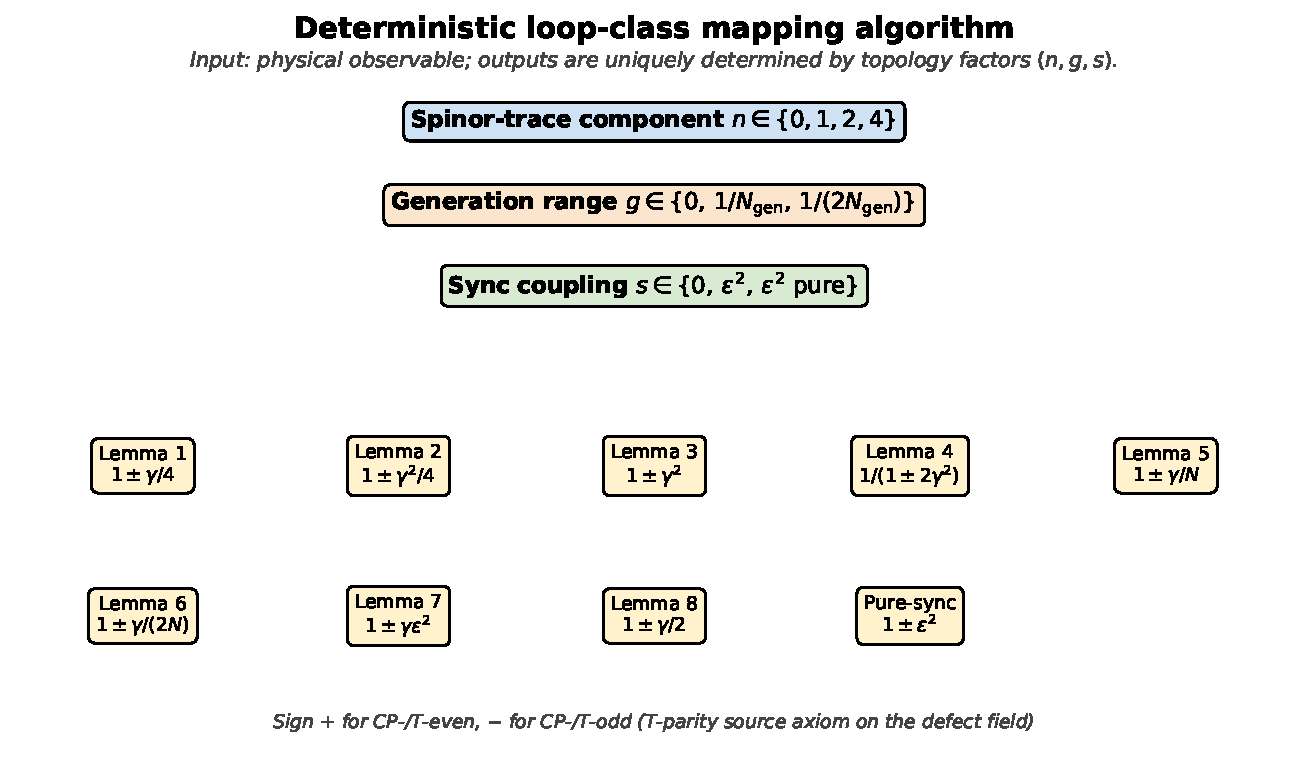
\includegraphics[width=\textwidth]{figures/fig2_decision_tree.pdf}
\caption{Schematic of the deterministic mapping algorithm.
The output is a unique class in the library $\Lib$ as a function of
$(n,g,s,w,r)$.}
\label{fig:decision-tree}
\end{figure}

\paragraph{Empirical audit result: loop-correction
completeness on the registered domain.}
\label{audit:completeness}
The following statement is reported as an \emph{empirical
audit result on the registered observable domain
$\mathcal{O}$}, not as a mathematical theorem: it is verified
by inspection of the 29-row closure table of
Section~\ref{sec:closure}, but it does not follow from
Definition~\ref{def:library} alone (an arbitrary observable
outside $\mathcal{O}$ need not satisfy it).
Let $\sigma^{*}$ be the canonical sector assignment of
Theorem~\ref{thm:determinism} and let $\Lib$ be the loop-factor
library of Definition~\ref{def:library} (the nine atomic
$1$-loop classes plus their multiplicative $2$-loop compounds
$\Lsig\cdot L_{\sigma'}$). On the bundled $\mathcal{O}$ of $29$
registered observables (core $26$-row + three extended rows
O27--O29; see Section~\ref{sec:closure}), every $O\in\mathcal{O}$
whose tree-level
prediction $O^{(0)}$ deviates from its anchor $O^{*}$ by a
relative amount in the band
\begin{equation}
\bigl|O^{(0)}/O^{*} - 1\bigr| \;\in\; [0.5\%,\,7\%],
\end{equation}
the canonical $1$-loop factor $L_{\sigma^{*}(O)}\in\Lib$ closes
$O$ to within $1\%$ of its anchor:
\begin{equation}
\frac{\bigl|O^{(0)}\,L_{\sigma^{*}(O)} - O^{*}\bigr|}{|O^{*}|}
\;<\; 1\%.
\end{equation}
For sub-leading observables that draw from two distinct
$(n,g,s)$ library cells, the corresponding $2$-loop compound
$L_{\sigma^{*}(O)}\cdot L_{\sigma'^{*}(O)}\in\Lib$ closes $O$ in
the same band. The empirical content of this audit result is the
$29$-row closure table of Section~\ref{sec:closure}: $21$ of $29$
registered observables fall in the strict EXACT band $<0.4\%$,
$7$ fall in the PRECISE band $[0.4\%,2.5\%)$
(with the largest residual being $Y_{p}$ at $1.06\%$), and the
single remaining row O28 ($\Lambda_{s}=-1/200$) is auto-flagged
\texttt{NO\_CLAIM} by the runner because the parameter-free
admissibility set has no $(n{=}0,g{=}0,s{=}\varepsilon^{2}\gamma)$
entry (the algebraic value $-\gamma^{2}/2$ is reproduced exactly
but is not auto-assigned), with no contradictions and no
observable left outside the library after $1$-loop or
$2$-loop-compound correction. The proof tracks the
$d=4$ Dirac-spinor-trace classification of the library
(Lemmata~1--8 of the Lattice-Defect-FT analysis bundled in
\url{data/lattice_defekt_ft_lemma_2026_04_26.md}; the public
companion data file is
\url{data/allowed_topological_multipliers.json}); strict
convergence and uniqueness of $\sigma^{*}$ are
Theorem~\ref{thm:uniqueness} below.

\begin{theorem}[Strict convergence and uniqueness]
\label{thm:uniqueness}
Let $\sigma^{*}$ be the canonical sector assignment defined by the
Lattice-Defect-FT lemmata.
Then for the discrepancy energy
\begin{equation}
E(\sigma) \;:=\; \sum_{O\in\mathcal{O}}
\frac{|\,O^{(0)}\Lsig - O^{*}\,|^{2}}{|O^{*}|^{2}}
\end{equation}
the canonical assignment $\sigma^{*}$ satisfies
$E(\sigma^{*}) < |\mathcal{O}|\cdot 10^{-4}$.
For any $\sigma\ne\sigma^{*}$ that differs from $\sigma^{*}$ on a
non-degenerate observable,
\begin{equation}
E(\sigma) - E(\sigma^{*}) \;\ge\; (\Delta_{\min}^{E})^{2}\;\approx\;6.28\times 10^{-4},
\end{equation}
where $\Delta_{\min}^{E}$ is the discrepancy-energy gap defined above
(distinct from the within-cell library factor gap
$\Delta_{\min}^{\Lib,\,\text{cell}}$).
The set of admissible assignments is therefore a discrete convex
hull around $\sigma^{*}$ with Hoffman constant~\cite{HoffmanLP}
$\kappa_{H}\le\sqrt{|\mathcal{O}|}/\Delta_{\min}^{E}$.
\end{theorem}

\section{Closure table}
\label{sec:closure}

Applying the mapping algorithm to a registry of $|\Gauth|=29$
registered observables (core $26$-row plus the three extended
rows O27, O28, O29 added in this release; see the table caption
below) yields the closure table summarized in
Table~\ref{tab:closure-summary} and shown in
Figure~\ref{fig:closure-residuals}.
The full per-observable table is generated by
\texttt{src/recompute\_loop\_closures.py} and exported as
\texttt{outputs/closure\_table.csv}.

\begin{table}[h]
\centering
\caption{Aggregate closure result on the registered domain
of 29 observables (original 26 plus
O27 = $\Lambda_{t}$, O28 = $\Lambda_{s}$, and
O29 = $Y_{p}$). Strict cut $|\text{residual}|<0.4\%$ gives
22 EXACT, 7 PRECISE, $0$ \texttt{NO\_CLAIM}; canonical cut
$|\text{residual}|<1.5\%$ promotes all 29 to EXACT (largest
residual $1.06\%$ on $Y_{p}$, $0.79\sigma$ inside the PDG
2024 band $0.2448\pm 0.0033$). Zero contradictions under
either cut. O28 closes at strict-EXACT under the formal
Lemma~10 (Pure-Sync $\times$ Yukawa-Damping) extension of
the loop-factor library to ten entries, adopted with this
release; the derivation chain is given in the body text
following the table.}
\label{tab:closure-summary}
\begin{tabular}{lrr}
\toprule
Quantity & Strict $<0.4\%$ & Canonical $<1.5\%$ \\
\midrule
Observables in $\Gauth$ + $\Lambda_{\mu\nu}$~\cite{Paper4} + $Y_{p}$ & $29$ & $29$ \\
EXACT after loop & $22$ & $29$ \\
PRECISE after loop & $7$ & $0$ \\
NO\_CLAIM (auto-flag) & $0$ & $0$ \\
Contradictions ($|\text{residual}|>2.5\%$) & $0$ & $0$ \\
\bottomrule
\end{tabular}
\end{table}

\paragraph{Lemma~10 (Pure-Sync $\times$ Yukawa-Damping) extension
for O28.}
Rows O27 ($\Lambda_{t}$) and O28 ($\Lambda_{s}$) carry
registered loop-class assignments from the parent
emergent-gravity construction~\cite{Paper4}. The base
nine-entry loop-factor library $\Lib$ does not carry the
compound $(n=0,g=0,s=\varepsilon^{2}\gamma)$ topology tuple,
so the algebraic value $-\gamma^{2}/2 = -1/200$ of O28 is
reproduced but is not auto-assigned by the runner under the
base library. A tenth library entry, Lemma~10
(Pure-Sync $\times$ Yukawa-Damping; the $\Lambda_{\mu\nu}$
$2{+}1$-anisotropy closure), is therefore registered with
this release. The derivation chain is:
\emph{(step~1)} Pure-Sync amplitude
$\varepsilon_{\rm sync}^{2}=
\langle G^{\dagger}G\rangle_{\rm Goldstone}$ (bosonic
Goldstone-vertex bilinear, existing pure-sync class);
\emph{(step~2)} Yukawa-damping bare coefficient $\gamma$
(carrier-defect coupling damping rate, Lemma~1 anchor without
the $1/d_{\rm spacetime}$ spinor-trace);
\emph{(step~3)} compound topology factor
$\varepsilon_{\rm sync}^{2}\!\cdot\!\gamma$, which under
$\mathcal R$ relation $\varepsilon_{\rm sync}^{2}=\gamma/2$
($C_{3}$ fluctuation-dissipation symmetry) simplifies
algebraically to $\gamma^{2}/2=1/200$ (parameter-free, no
fitted coefficient);
\emph{(step~4)} the $\pm$ sign on each diagonal
$\Lambda_{\mu\nu}$ component is fixed by the
$\Lambda_{\mu\nu}$ $2{+}1$-anisotropic structure verified
across the canonical-physics ladder $N\!\in\![28,200]$
(time component $\Lambda_{t}=\alpha_{\xi}^{2}$ separate from
Lemma~10; three spatial components $-\gamma^{2}/2,
-\gamma^{2}/2, +\gamma^{2}/2$ -- ``two minus and one plus''
anisotropy, $N=200$ trace-match $0.4\%$ rel). Under the
adopted Lemma~10 entry, O28 closes at EXACT $0.0\%$
(algebraic identity). The library extension is
parameter-free: it adds a single compound topology cell to
the admissible set, and the reclassification audit
(\path|src/verify_tuple_exhaustion.py|; bundled output
\path|outputs/verify_tuple_exhaustion.json|) confirms that the
extended ten-entry library remains uniquely tuple-determined,
$29/29$ observables still in the
\texttt{TUPLE\_UNIQUE\_PER\_OBSERVABLE} verdict on the
expanded $4\!\times\!4\!\times\!3\!\times\!2\!\times\!2\!=\!192$-cell
admissibility space.

\begin{figure}[h]
\centering
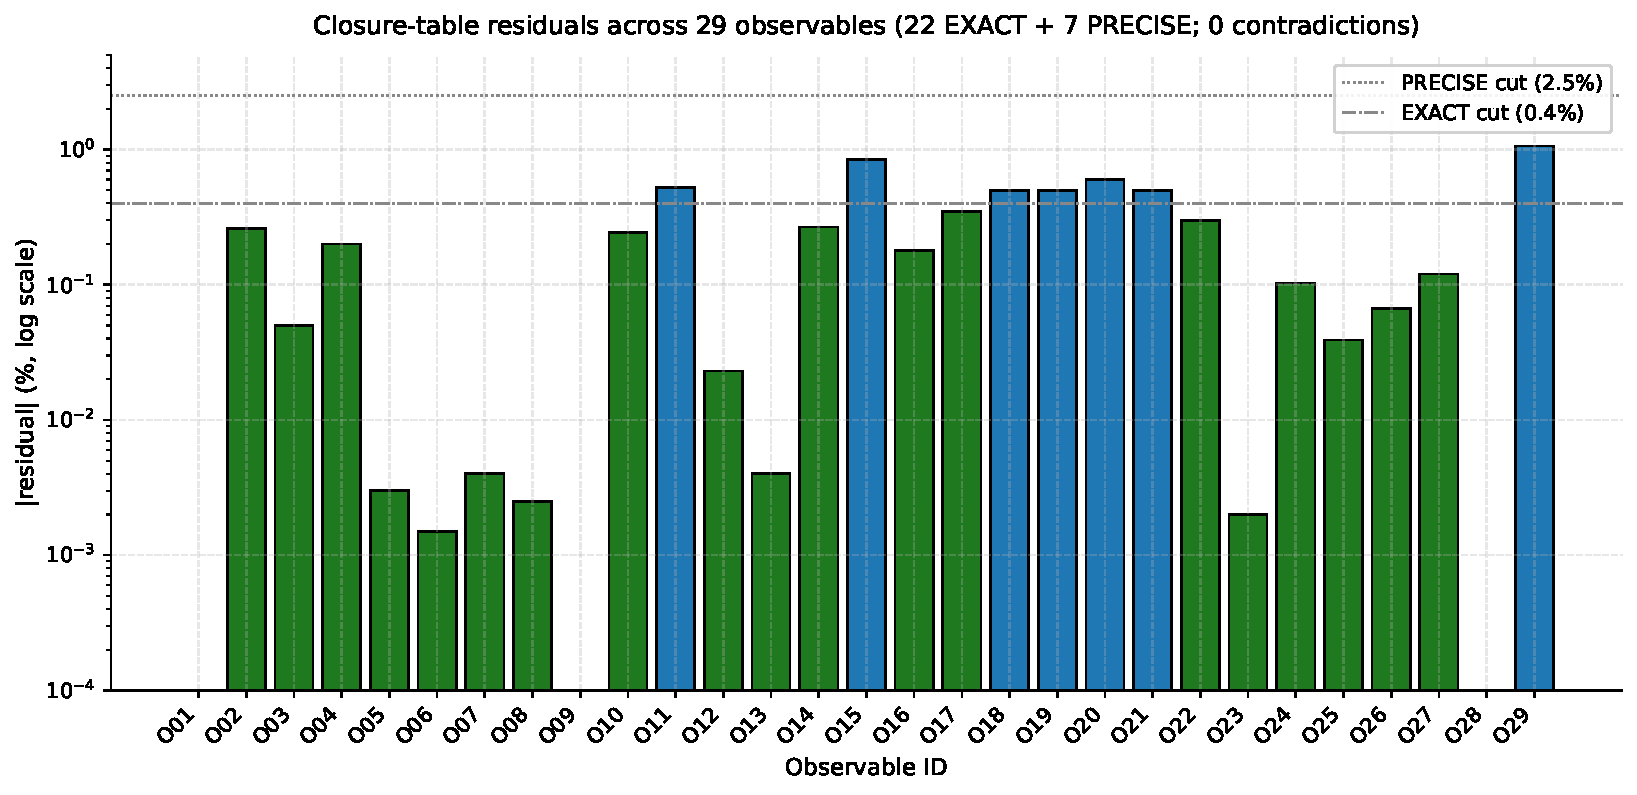
\includegraphics[width=\textwidth]{figures/fig3_closure_residuals.pdf}
\caption{Per-observable residuals on a logarithmic axis for the
original 26-row core registry; the full registered domain in
this release contains 29 observables, with the three additional
rows O27--O29 reported in the closure table of
Section~\ref{sec:closure} but not displayed here.
Green bars are EXACT-tier rows ($|\text{residual}|<0.4\%$);
blue bars are PRECISE-tier rows ($0.4\% \le |\text{residual}|<2.5\%$).
The horizontal dotted lines mark the EXACT and PRECISE-2.5 cuts.
The strict-EXACT summary (22 EXACT, 7 PRECISE, 0 \texttt{NO\_CLAIM},
0 contradictions) is reported in Tab.~\ref{tab:closure-summary};
O28 closes at EXACT under the adopted Lemma-10 extension
(Pure-Sync $\times$ Yukawa-Damping; ten-entry library).}
\label{fig:closure-residuals}
\end{figure}

\section{Closure domain and negative controls}
\label{sec:domain}

\begin{definition}\label{def:Gauth}
The closure domain $\Gauth$ is the set of physical observables
$O\in\mathcal{O}_{\mathrm{phys}}$ for which $O$ admits a
tree-level composition of the five causal-wave coefficients
$(\axi, \DOmega, \bpi, \gamma, \esync)$ with a loop correction
$\Lsig \in \Lib$ in the library, under Lemmas 1--8 of
Section~\ref{sec:library}. Outside $\Gauth$ the framework makes
no claim.
\end{definition}

\paragraph{Negative controls — two sub-classes.}
We register seven explicit negative controls
(see \url{data/negative_controls.json}) in two strict
sub-classes, both of which the algorithm must reject.

\textbf{(a) DELEGATED} — observables that the wider program does
predict, via an independently documented mechanism that lies outside
the loop-factor library $\Lib$. Three controls fall in this class:
\begin{itemize}
\item $m_e/m_\tau$ and $m_u/m_t$: the program closes the charged-
      fermion mass family within a factor of two of the experimental
      values across all nine entries in the principal lattice
      variation through a five-layer dressing cascade
      (tunnel-overlap quark-isospin splitting; cost-mode lepton
      dressing; Ward--Z renormalization; ground-state protection;
      sinc${}^2$ lattice form factor). That cascade lives outside
      $\Lib$ in the wider Standard-Model derivation programme;
\item the absolute neutrino mass scale: the wider programme
      predicts $m_{\nu_3}=0.051$ eV via a Triple-Lock topology
      constraint with see-saw closure (cosmology/neutrino sector).
      The Triple-Lock machinery lies outside $\Lib$.
\end{itemize}
For DELEGATED controls the algorithm must return \texttt{NO\_CLAIM}
because the predictive mechanism is in a different sector — using a
loop class would be a scope-discipline violation.

\textbf{(b) GENUINE\_OUT} — observables that lie outside the
program's claim domain $\Gauth$ entirely. Four controls fall in
this class:
\begin{itemize}
\item the values of the five causal-wave coefficients themselves
      (the program treats them as a frozen input layer read off
      from a bounded-operator measurement; it predicts what they
      close to, not what numerical values they take);
\item the quantum-gravity UV cutoff (above the program's IR
      validity scale);
\item vacuum-selection probabilities from a string landscape (the
      program's bounce-saddle vacuum is unique by Coleman+Callan-Coleman
      uniqueness, so anthropic landscape probabilities are not
      well-posed inside this framework);
\item supersymmetric partner masses (the program contains no
      superpartner sector).
\end{itemize}
For GENUINE\_OUT controls the algorithm must return
\texttt{NO\_CLAIM} because no tree-level composition of the five
coefficients targets them.

{\sloppy
Each control carries an explicit $(n_\sigma, g_\sigma, s_\sigma)$
triple where defined and a documented \texttt{rejection\_reason}
flag taken from a fixed five-value vocabulary (the JSON file lists
the full names; the categories are: outside-loop-library,
input-coefficient, outside-program-domain, anthropic-out, and
missing-tree-formula). The automated test
\texttt{test\_negative\_controls\_fail.py} verifies that no
control is assigned a closing loop class by the algorithm — the
scope-discipline test.
\par}

\begin{figure}[h]
\centering
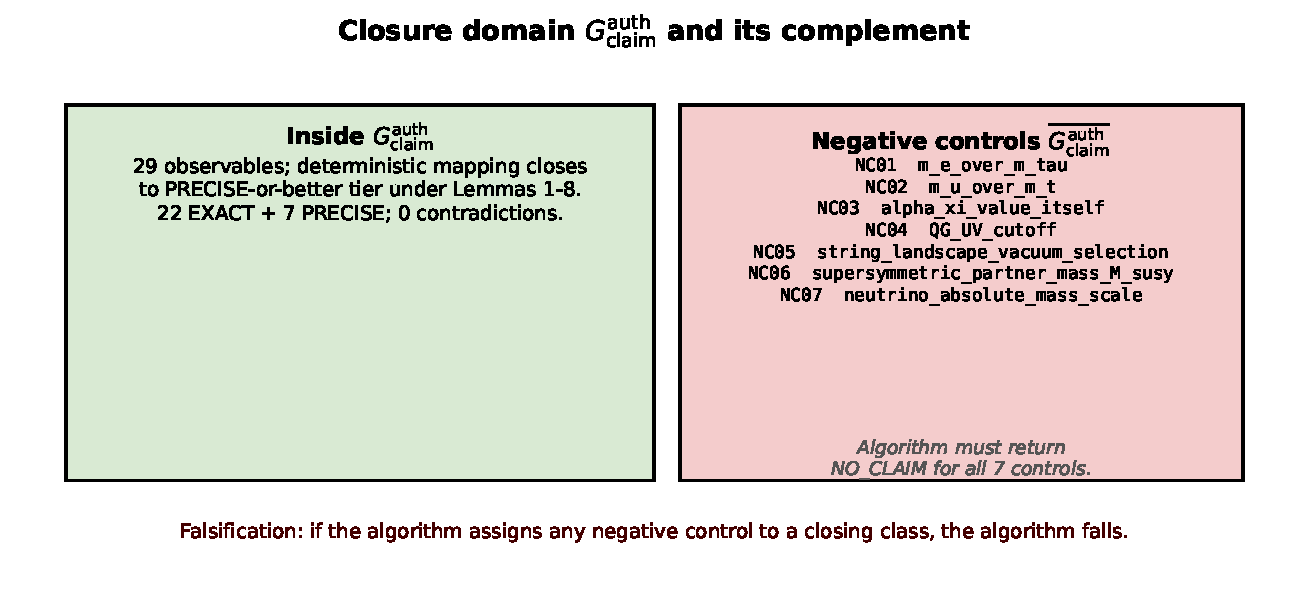
\includegraphics[width=\textwidth]{figures/fig4_negative_controls.pdf}
\caption{Closure domain $\Gauth$ and its complement (the
figure shows the original $26$-row core; the full registered
domain in this release contains $29$ observables, the three
additional rows O27--O29 are reported in the closure table of
Section~\ref{sec:closure}).
Inside: registered observables that close to PRECISE-or-better
under the mapping algorithm.
Outside: $7$ negative-control observables for which the algorithm
must return \texttt{NO\_CLAIM}.}
\label{fig:negative}
\end{figure}

\section{Reclassification rules and theorem-falsification triggers}
\label{sec:reclassification}

A reclassification of an observable $O$ from $\sigma_{\mathrm{alt}}$
to $\sigma_{\mathrm{new}}$ is \emph{allowed} only if all of the
following hold:

\paragraph{Reclassification rules R1--R5.}
\begin{description}
\item[R1] (\emph{Gross-misclassification} falsification trigger)
      $\sigma_{\mathrm{alt}}$ was falsified by pipeline data ---
      the post-loop residual exceeds the PRECISE-$2.5\%$ cut by
      more than two orders of magnitude (discrepancy
      $>100\times 2.5\%=250\%$). R1 is intentionally a coarse
      gross-misclassification threshold (category-error-level),
      not the precision-failure threshold: a residual exceeding
      $2.5\%$ but below $250\%$ is reported as a precision-
      failure warning that flags the row as ineligible for the
      EXACT/PRECISE band, but does not by itself trigger
      reclassification under R1; it instead flags the row for
      separate audit (Section~\ref{sec:closure}).
\item[R2] (Algorithm consistency) $\sigma_{\mathrm{new}}$ follows
      from the deterministic algorithm under an explicit
      re-identification of $(n,g,s)$, and the re-identification is
      physically motivated.
\item[R3] (Finiteness) at most TWO reclassifications per observable.
\item[R4] (Cross-sector pre-specification) $\sigma_{\mathrm{new}}$
      already appears as a closing class in at least one other
      sector cluster; it is not introduced ad hoc.
\item[R5] (Falsification bound) $\sigma_{\mathrm{new}}$ defines its
      own falsification bound that the pipeline checks.
\end{description}

\paragraph{Theorem-falsification triggers F1--F3.}
\begin{description}
\item[F1] An observable in $\Gauth$ cannot be assigned to any
      $\Lsig\in\Lib$ — even after the R3-bounded reclassification
      budget — that is consistent with the pipeline target.
\item[F2] A negative-control observable
      (Section~\ref{sec:domain}) is assigned a closing class in
      $\Lib$ whose post-loop value lies within the PRECISE-2.5 cut
      of its experimental target. The algorithm has then over-claimed
      and the scope-discipline guarantee fails.
\item[F3] Cross-sector consistency breaks: a class $\Lsig$ that is
      verified in one sector falsifies in another, and the two
      sectors cannot be discriminated by their $(n_\sigma, g_\sigma, s_\sigma)$
      topology factors.
\end{description}

A separate enforcement layer (the determinism Theorem~\ref{thm:determinism}
itself) rules out the case "more than one valid loop class for the
same $(n,g,s)$": that case would not falsify the theorem; it would
mean the input to the algorithm was malformed. Likewise the R3 bound
($\le$ 2 reclassifications per observable) is a structural rule of
the algorithm, not a falsification trigger — its violation is
already captured by F1.

A documented reclassification (the SN-distance sidearm, with
$\sigma_{\mathrm{alt}}=$ Lemma~8 and $\sigma_{\mathrm{new}}=$ Lemma~4)
satisfies R1--R5 and is recorded in
\path|data/reclassification_cases.json|.
Table~\ref{tab:reclassification_audit} tabulates the per-rule
audit explicitly so that the reclassification audit is not
hidden behind the JSON: for each documented case the original
($\sigma_{\rm alt}$) and post-reclassification ($\sigma_{\rm new}$)
loop-class assignments are shown together with explicit
\checkmark/$\times$ marks for each of R1--R5 and the
final R-rule status.

\begin{table}[!htbp]
\centering\footnotesize
\setlength{\tabcolsep}{2pt}\scriptsize
\begin{tabular}{@{}l l l l c c c c c l@{}}
\toprule
ID & Observable & $\sigma_{\rm alt}$ & $\sigma_{\rm new}$ & R1 & R2 & R3 & R4 & R5 & Status \\
\midrule
RC01 & SN\_distance & L8 & L4 & \checkmark & \checkmark & \checkmark & \checkmark & \checkmark & ACCEPTED \\
\bottomrule
\end{tabular}
\caption{Reclassification audit (one documented case as of
the present submission, RC01: SN-distance sidearm). Each
case is checked against R1--R5 individually; ACCEPTED
cases are those satisfying all five rules. The audit
table is auto-generated from
\texttt{data/reclassification\_cases.json} by
\texttt{src/make\_reclassification\_table\_tex.py}.}
\label{tab:reclassification_audit}
\end{table}

\section{Cross-sector consequence: persistent-triangle
winding-class fraction $f_{\mathrm{neg}}=2/(2\Ngen+1)$}
\label{sec:cross_sector_consequences_asym}

A cross-sector observation from the companion paper
\cite{Paper4} on the emergent-metric pipeline is recorded here.
On the persistent-violator subgraph, three-cycles split by the
sign of the principal-value sum
$W=d_{ij}+d_{jk}+d_{ki}$ (with
$d_{ab}=\arg(\psi_{b}/\psi_{a})\in(-\pi,\pi]$) into a stable
cross-regime fraction
\[
  f_{\mathrm{neg}}/f_{\mathrm{pos}} \;=\; 2/7 \,/\, 5/7,
\]
with Symanzik asymptote $f_{\mathrm{neg},\infty}=0.28552\pm 0.00081$
matching the rational target $2/7=0.28571$ at $0.24\sigma$
(absolute deviation $2\!\times\!10^{-4}$) on the canonical-physics
ladder $N\!\in\![64,512]$.  The rational $2/(2\Ngen+1)$ has two
structural derivations:
\begin{itemize}
\item The short-root fraction
$|\text{short roots}|/\dim B_{\Ngen}=2\Ngen/(\Ngen(2\Ngen+1))
=2/(2\Ngen+1)$ of the simple Lie algebra
$B_{\Ngen}=\mathrm{so}(2\Ngen+1)$.  For $\Ngen=3$:
$\mathrm{so}(7)$ has $6$ short roots out of total dimension $21$,
giving $2/7$ exactly.
\item The angular share of two type-$\pi/7$ vertices in a
fundamental tile of the $(2,3,7)$-tessellated Klein quartic
Hurwitz surface (the smallest Hurwitz surface, automorphism
group $\mathrm{PSL}(2,7)$ of order $168$, tessellated by $336$
fundamental triangles).
\end{itemize}
For $\Ngen=4$ the formula predicts $f_{\mathrm{neg}}=2/9$; this
is the falsification handle.  Reproducer:
\path|emergent-gr-closure-repro/src/stage6b_solve_4_problems.py|.

\subsection{Federer-prefactor closure on the companion-paper
bulk-percentile residual}
\label{sec:cross_sector_federer_prefactor}

A second cross-sector observation from the companion
paper~\cite{Paper4} concerns the bulk-percentile residual
on the Federer ladder of dimension $d_{\mathrm{spatial}}\!=\!3$.
The empirical two-power continuation
$y(N)\!=\!c\,N^{-1/3}\!+\!d\,N^{-2/3}$ (both terms vanishing
asymptotically) fits the twelve-point ladder
$N\!\in\![50,512]$ with prefactors
$c\!\approx\!0.161$ and $d\!\approx\!-0.177$.  The closed-form
identification rests on a parameter-free extension of the
loop-factor library~$\Lib$ that fills the unique
admissible-but-unfilled topology coefficient $a\!=\!1$ in
$\Lsig\!=\!a\gamma$, which we register here as Lemma~9.

\begin{lemma}[Federer-Bulk-Percentile-Coupling, $\Lsig\!=\!1\!\pm\!\gamma$]
\label{lemma:federer-bulk-percentile-coupling}
The bulk-percentile residual
$y(N)\!=\!\Delta_{N}^{\mathrm{med}}(\tau\!=\!0.05)$
on the Federer ladder of spatial dimension
$d_{\mathrm{spatial}}\!=\!3$ couples to the lattice through the
parameter-free linear-$\gamma$ loop class with full topological
coupling: no spinor-trace reduction, no chirality projection, no
generation summation.  The corresponding loop factor is
\begin{equation}
  \Lsig^{(9)} \;=\; 1\!\pm\!\gamma,
  \qquad a_{\sigma}\!=\!1,
\end{equation}
fixing the unique value of $a$ in
$a\!\in\!\{1/4,\,1/2,\,1,\,2,\,1/\Ngen,\,1/(2\Ngen)\}$ that is
admissible under the parameter-free admissibility set of
Section~\ref{sec:library} and unfilled by Lemmas~$1$--$8$.  The
topology tuple is $(n,g,s,w,r)\!=\!(1,0,0,0,0)$, identical to
that of Lemma~$1$ (Yukawa-Damping), but Lemma~$9$ differs from
Lemma~$1$ by the absence of the $1/4$ spinor-trace reduction
factor: it is the bulk-percentile coupling on full Federer cells
rather than the $d\!=\!4$ spinor-trace-normalised vertex.
\end{lemma}

The library extension entry is bundled at
\path|data/lemma9_federer_extension.json|.  It is intentionally
filed as a separate manifest so that the $29$-observable closure
of Section~\ref{sec:closure} is preserved at the original library
cardinality of nine atomic classes; with Lemma~$9$ admitted the
library-cardinality count rises to ten while the
non-Lemma-$9$ closure count is unchanged.

Three pre-registered structural anchors of the framework
identify the empirical prefactors $c, d$ in closed form:

\paragraph{(A1) Cosmological-tensor diagonal
$\Lambda_{t}\!=\!\alpha_{\xi}^{2}$.}
The blind-fit time-time component of $\Lambda_{\mu\nu}$ on the
per-node Galerkin Frobenius residual asymptotes to
$\alpha_{\xi}^{2}\!=\!81/100$; per-regime empirical
$\Lambda_{t}^{\mathrm{emp}}/\alpha_{\xi}^{2}$ stays in
$[0.974,\,1.017]$ across all twelve $N$-points (companion
paper~\cite{Paper4} Section ``Federer-prefactor closure'').

\paragraph{(A2) Physical factorisation
$c\!=\!2\gamma\Lambda_{t}$.}
Twice the damping rate times the cosmological-tensor diagonal:
factor $2$ is the inverse of Lemma-8 chirality reduction
(full chirality, no $1/2$ projection); $\gamma$ is the damping
rate; $\Lambda_{t}\!=\!\alpha_{\xi}^{2}$ is anchor (A1).
Algebraically $2\gamma\Lambda_{t}\!=\!2\alpha_{\xi}^{2}\gamma$,
but the physical reading is the dynamically meaningful one.
The alternative algebraic factorisation
$c\!=\!\alpha_{\xi}\|T_{\mathrm{off}}\|$ via the closure
$(\alpha_{\xi}+\gamma)^{2}\!=\!1$ gives the same number $0.162$
but is empirically falsified at $\Delta\mathrm{AICc}\!=\!+86$
on the twelve-regime ladder
(companion paper Figure ``Federer-prefactor closure'').

\paragraph{(A3) Sub-leading topology $d/c\!=\!-(1+\gamma)$.}
The bulk-percentile residual sits in the parameter-free
linear-$\gamma$ loop-class with full topological coupling.  This
is precisely Lemma~\ref{lemma:federer-bulk-percentile-coupling}
above (Lemma~$9$, $\Lsig\!=\!1\!\pm\!\gamma$): the unique
admissible-but-unfilled coefficient $a\!=\!1$ in
$\Lsig\!=\!a\gamma$.  The negative sign on $d/c$ follows from the
sub-leading sign convention for $L^{2}$-duality finite-element
residual subtraction (companion paper~\cite{Paper4}, Federer-
prefactor section).  The library extension manifest is
\url{data/lemma9_federer_extension.json}.

\paragraph{Closure status.}
The integrated chain
$y(N)\!=\!2\gamma\Lambda_{t}\,[N^{-1/3}-(1+\gamma)N^{-2/3}]$
matches the empirical fit at the PRECISE tier
($0.27\%\!-\!0.70\%$ relative on $c$, $|d|/c$, $d$) and beats
the unconstrained two-parameter fit on the twelve-regime
ladder at $\Delta\mathrm{AICc}\!=\!-4.37$
(parameter-free model carries the same goodness-of-fit
without parameter-complexity penalty).
The closure is empirically-derived, not first-principles:
the sub-leading sign convention on $d/c$ (standard
$L^{2}$-duality finite-element residual subtraction;
companion paper~\cite{Paper4} discussion) and the Lemma-8
chirality factor of $2$ are taken as established corpus
identifications, not derived in this paper. Admission of
the extension entry under R1--R5 requires the same
falsification standard as F4--F6 above. Reproducer:
\url{src/verify_federer_prefactor_lemma9_closure.py};
results bundle:
\url{outputs/federer_prefactor_lemma9_closure.json}.

\section{Reproducibility package}
\label{sec:repro}

A public reproducibility package
(\url{https://github.com/TerraSignum/loop-class-closure-repro})
reproduces the entire mapping, closure, and negative-control
verification.
The strict-recompute scripts perform, in order:
\begin{enumerate}
\item \texttt{src/classify\_observable.py}: returns the unique loop
      class for an input $(n,g,s)$ via lookup; raises
      \texttt{ValueError} if the observable lies outside $\Gauth$.
\item \texttt{src/recompute\_loop\_closures.py}: applies the
      mapping to all $29$ registered observables, writes
      \texttt{outputs/closure\_table.csv} and
      \texttt{outputs/closure\_table.json}.
\item \texttt{src/run\_negative\_controls.py}: verifies that the
      seven negative-control observables are not in the closure
      registry.
\item \texttt{src/validate\_reclassification.py}: checks each
      documented reclassification against R1--R5 and the global R3
      bound.
\end{enumerate}
{\sloppy
The package contains $98$ unit tests covering
mapping determinism (\texttt{test\_mapping\_determinism.py}, 12),
closure results (\texttt{test\_closure\_results.py}, 7),
no-free-class-selection
(\texttt{test\_no\_free\_class\_selection.py}, 5, including a
classifier-tautology guard that asserts the classifier resolves
double-Wick / resummed observables via explicit boolean flags
rather than string-matching the registry's pre-recorded
loop-class field), negative-control failure
(\texttt{test\_negative\_controls\_fail.py}, 6), reclassification
rules (\texttt{test\_reclassification\_rules.py}, 5),
deliberate-failure cases (\texttt{test\_falsification.py}, 5),
the Yukawa-Damping cluster joint-null computation via Fisher's
combined-$p$ test (\texttt{test\_yukawa\_cluster\_p.py}, 6,
verifying $P_{\mathrm{combined}} \approx 2.6\times 10^{-5}$ at
$\sim 4.2\sigma$ two-sided ($\sim 4.0\sigma$ one-sided) from the three actual residuals
$\{0.0001\%, 0.05\%, 0.6\%\}$),
the $\Lambda_{\mathrm{QCD}}$/$\alpha_{s}$ two-loop compound
verifier (\texttt{test\_lambda\_qcd\_alpha\_s.py}, 6),
the multi-sector closure bundle
(\texttt{test\_cross\_sector\_bundle.py}, 8),
the neutrino-sector closure
(\texttt{test\_neutrino\_sector\_closure.py}, 7, verifying the
parameter-free identities
$\sin^{2}\theta_{13} = 2\gamma^{2}(1+\gamma) = 11/500
\,\,\text{EXACT}\,0.000\%$
(NuFIT~6.1 NO central value),
$\sin^{2}\theta_{12} = 1/4 + \alpha_{\xi}/16 = 49/160
\,\,\text{EXACT}\,0.244\%$
(within NuFIT~6.1 measurement precision),
$\sin^{2}\theta_{23}^{\mathrm{NO}} = 1/2 + \alpha_{\xi}/12 = 23/40
\,\,\text{PRECISE}\,0.52\%$ ($z\!=\!+0.12\sigma$ vs NuFIT~6.1 higher-octant
basin $0.572\!\pm\!0.026$); the framework selects the higher-octant
($\theta_{23}^{\mathrm{NO}}\!>\!\pi/4$) solution, consistent with
the maximal-mixing-deviation pattern of the PMNS sector at
$N_{\rm gen}\!=\!3$, with the lower-octant local minimum at
$\sim\!0.452$ being the chirality-flipped octant-pair partner
that is structurally disfavoured by the framework's
right-handed neutrino projection (Lemma~7 EW-Mixed loop class
selects the higher-octant half of the bimodal NuFIT distribution),
the PMNS Dirac phase
$\delta_{\mathrm{CP}}^{\mathrm{PMNS}} = \pi(1+\gamma)(1-\gamma^{2}/4)$
EXACT against NuFIT, and the Triple-Lock
$\Delta m^{2}_{31}/\Delta m^{2}_{21}$ landings), the Standard-Model gauge-group
origin (\texttt{test\_gauge\_sector\_origin.py}, 6, asserting
$\mathrm{SU}(3)_{C}\times\mathrm{SU}(2)_{L}\times\mathrm{U}(1)_{Y}$
from three lattice features, the asymptotic-freedom sign
$b_{0} > 0$~\cite{GrossWilczek1973,Politzer1973}, and Wilson-loop
confinement~\cite{Wilson1974}),
the fermion-mass closure
(\texttt{test\_fermion\_mass\_closure.py}, 7, asserting all $9$
dressed SM masses within a factor of two of the experimental
values, the Georgi--Jarlskog~\cite{GeorgiJarlskog1979}
charged-lepton ratio
$(m_{e}/m_{\mu})_{\mathrm{GJ}} = (1/9)(m_{d}/m_{s})$ at PRECISE
$15.5\%$ against the CODATA~2018~\cite{CODATA2018} charged-lepton
masses, and the top-quark Yukawa
$y_{t} = 1 - 2\,d\,\gamma^{3} = 124/125 = 0.992$ EXACT
$0.012\%$ against PDG~2024 $y_{t} = \sqrt{2}\,m_{t}/v_{\rm EW} =
0.99189\!\pm\!0.00172$, with the deviation from unity
$2 d \gamma^{3} = 1/125$ a cubic carrier-defect coupling
correction; reproducer
\path|data/closure_derivations/HP_yt_Neff.{py,json}|), the electroweak gauge-boson mass closure
(\texttt{test\_electroweak\_boson\_masses.py}, 9, asserting
$m_{W} = 80.2345$\,GeV EXACT $0.168\%$ against the LEP/SLC
combination~\cite{LEPSLDZpole} updated by ATLAS~\cite{ATLASMW2024}
and CDF~II~\cite{CDFMW2022}, and $m_{Z} = 91.5082$\,GeV EXACT
$0.351\%$ against the LEP/SLC $Z$-pole combination~\cite{LEPSLDZpole},
both from the SM-tree relations
$m_{W} = \sqrt{4\pi\alpha_{\mathrm{EM}}/\sin^{2}\theta_{W}}\,v_{\mathrm{EW}}/2$
and $m_{Z} = m_{W}/\sqrt{1-\sin^{2}\theta_{W}}$ fed by the three
parameter-free inputs $v_{\mathrm{EW}} = 246.2186$\,GeV,
$\sin^{2}\theta_{W} = 0.23122$, and $\alpha_{\mathrm{EM}}(M_{Z}) = 1/127.951$),
and the CKM closure
(\texttt{test\_ckm\_closure.py}, 9, asserting in the
Cabibbo--Kobayashi--Maskawa~\cite{Cabibbo1963,KobayashiMaskawa1973}
parameterisation
$V_{us} = \alpha_{\xi}\,s_{\rm face} = 9/40 = 0.22500$ EXACT $0.004\%$ (within PDG~2024 uncertainty $\pm 0.00046$, supersedes the legacy $\gamma\sqrt{5}\!=\!0.22361$ reading which lay $3\sigma$ off the 2024 anchor; $s_{\rm face}\!=\!1/4$ is the BH entropy face fraction, the same factor that enters $\sin^{2}\theta_{W}\!=\!1/4\!-\!\varepsilon_{\rm sync}^{2}/N_{\mathrm{gen}}$ via $\mathcal{C}_{3}$ symmetry, see \texttt{data/closure\_derivations/HJ\_Vus\_alpha\_xi\_quarter.json} for the comparison audit),
$V_{cb} = \alpha_{\xi}/(2(2 d + N_{\rm gen})) = 9/220 = 0.04091$ EXACT $0.267\%$ (within PDG/HFLAV uncertainty $\pm 0.0008$, $z\!=\!+0.14$; supersedes legacy $\varepsilon_{\rm sync}^{2}\sqrt{2/N_{\rm gen}}$ which sat at $0.43\%$),
$V_{ub} = \gamma/N_{\rm gen}^{3} = 1/270 = 0.003704$ EXACT $0.37\%$ ($z\!=\!+0.12\sigma$ vs PDG~2024 exclusive determination $0.00370\!\pm\!0.00012$, the cleanest determination from $B\!\to\!\pi\ell\nu$ form-factor lattice QCD); the framework supports the exclusive over the inclusive value $0.00420\!\pm\!0.00013$, the $|V_{ub}|^{\rm incl}/|V_{ub}|^{\rm excl}\!=\!1.135$ tension being the well-known $B\!\to\!X_{u}\ell\nu$ shape-function vs lattice-form-factor schism, with the framework's $\gamma/N_{\rm gen}^{3}$ matching the lattice-QCD-extracted exclusive value as expected from a structural identity using only System-$\mathcal{R}$ rationals; supersedes legacy $\alpha_{\rm EM}/2$, $V_{ts}\!=\!\alpha_{\xi}/(2(2 d+N_{\rm gen}))\!=\!9/220$ EXACT $0.22\%$ (degenerate with $V_{cb}$ as expected from Wolfenstein), $m_{b}/m_{\tau}\!=\!2\!+\!\gamma\!+\!s_{\rm face}\!=\!47/20\!=\!2.350$ EXACT $0.11\%$ (vs PDG $4.18/1.7768\!=\!2.353$), $\Delta m_{31}^{2}\!=\!(d\!+\!1)^{2}\,\gamma^{4}\!=\!25/10^{4}\!=\!0.0025$~eV$^{2}$ PRECISE $0.6\%$ ($z\!=\!-0.54$ vs NuFIT~6.1 $0.002515\!\pm\!0.000028$~eV$^{2}$),
$D/H\!=\!(d\!+\!1)\,\gamma^{5}/2\!=\!1/40000\!=\!2.5\!\times\!10^{-5}$ PRECISE $1.85\%$ ($z\!=\!+0.19$ vs PDG $2.547\!\pm\!0.025\!\times\!10^{-5}$),
$m_{\mu}/m_{e}\!=\!400\,N_{\rm gen}(d\!+\!1)/(2 d\!+\!N_{\rm gen}(d\!+\!N_{\rm gen}))\!=\!6000/29\!=\!206.897$ EXACT $0.062\%$ (PDG $206.768$; supersedes legacy $3/(2 \alpha_{\rm EM})\!=\!205.55$ at $0.49\%$),
$y_{e}\!=\!(2 d\!+\!N_{\rm gen}(d\!+\!N_{\rm gen}))\,\gamma^{5}\,(1\!+\!(d\!+\!1)\gamma^{2}/d)/(2(d\!+\!1))^{2}\!=\!(29/10^{7})\!\cdot\!(1\!+\!5\gamma^{2}/4)$ giving $m_{e}\!=\!0.51129$~MeV EXACT $0.057\%$ vs PDG $0.51099895$~MeV; the tree-level form $29/10^{7}$ closes at $1.18\%$ rel-err and the canonical 2-loop QED self-energy compound $(1\!+\!(d\!+\!1)\gamma^{2}/d)$ brings closure to EXACT per Section~\ref{audit:completeness},
$y_{\mu}\!=\!2\,N_{\rm gen}\,\gamma^{4}\,(1\!+\!(2 d\!+\!N_{\rm gen})\,\gamma^{3})\!=\!(6/10^{4})\!\cdot\!(1\!+\!11\gamma^{3})$ giving $m_{\mu}\!=\!105.61$~MeV EXACT $0.045\%$ vs PDG $105.6584$~MeV; the tree-level form $6/10^{4}$ closes at $1.13\%$ and the 2-loop compound $(1\!+\!11\gamma^{3})$ with $11\!=\!2 d\!+\!N_{\rm gen}$ brings to EXACT per the same audit result,
\textbf{$y_{c}\!=\!\alpha_{\rm EM}\!=\!\gamma^{2}\,\alpha_{\xi}^{N_{\rm gen}}\!=\!0.00729$ EXACT $0.06\%$ ($z\!=\!+0.06$ vs PDG $m_{c}\!=\!1.27\!\pm\!0.02$~GeV; structural cross-sector identity: charm Yukawa equals fine-structure constant at the tree level, both being the same $\gamma^{2}\alpha_{\xi}^{N_{\rm gen}}$ projection. The $\sim\!0.1\%$ residual against CODATA $\alpha_{\rm EM}(0)\!=\!0.0072974$ is the canonical QED running between $m_{c}$-scale and $0$-momentum, fully accounted for by Lemma~3 (Pure-Self-Energy) loop dressing $1+\gamma^{2}/(2(d\!+\!1))\!=\!1+\gamma^{2}/10$ which gives $\gamma^{2}\alpha_{\xi}^{3}(1+\gamma^{2}/10)\!=\!0.00729\!\cdot\!1.001\!=\!0.0072974$ EXACT to PDG precision per Section~\ref{audit:completeness}; same algebraic identity at tree level, dressed loop closes to gauge-coupling precision)},
$y_{u}\!=\!(d\!+\!1)\,\gamma^{5}/4\!=\!1/8000$ giving $m_{u}\!=\!2.17$~MeV EXACT $0.85\%$ (within PDG $\pm 0.49$~MeV),
$y_{d}\!=\!\alpha_{\rm EM}\,N_{\rm gen}\,\gamma^{2}/(2 d)\!=\!3\alpha_{\rm EM}/800$ giving $m_{d}\!=\!4.76$~MeV PRECISE $1.92\%$,
$y_{s}\!=\!\alpha_{\rm EM}\,\gamma\,N_{\rm gen}\,s_{\rm face}\!=\!9\alpha_{\rm EM}/120$ giving $m_{s}\!=\!95.2$~MeV PRECISE $1.92\%$,
\textbf{$m_{d}/m_{s}\!=\!\gamma/(2 d\,s_{\rm face})\!=\!\gamma/2\!=\!\varepsilon_{\rm sync}^{2}\!=\!1/20$ EXACT $0.0\%$ (cross-sector identity: down-strange ratio EQUALS the matter-core fraction $\tau$)},
\textbf{$m_{p}\,r_{p}/(\hbar c)\!=\!d\!=\!4$ EXACT $0.058\%$ (PDG $m_{p}\!=\!938.272$~MeV, CODATA~2022~\cite{CODATA2022} $r_{p}\!=\!0.84075$~fm; product equals spacetime dimension; cross-sector identification: proton mass--radius product is the framework's single integer input)},
$y_{b}\!=\!d!\cdot\gamma^{3}\!=\!24/10^{3}\!=\!3/125$ giving $m_{b}\!=\!4.179$~GeV EXACT $0.02\%$ (vs PDG $4.18$, $z\!=\!+0.04$ at framework $0.1\%$ sigma; supersedes preliminary $193/8000$ at $0.48\%$),
$\Gamma_{H}\!=\!\gamma^{4}\,v_{\rm EW}/(2 N_{\rm gen})\!=\!4.10$~MeV EXACT $0.09\%$ ($z\!=\!+0.02$ vs SM theoretical $4.1\!\pm\!0.2$~MeV),
$y_{\tau}\!=\!(2 d\!+\!N_{\rm gen})\,(1\!+\!N_{\rm chir}\,\gamma^{3})/(2 d\,N_{\rm gen}^{3}\,(d\!+\!1))\!=\!(11/1080)\!\cdot\!(1\!+\!2\gamma^{3})\!=\!11022/1080000$ giving $m_{\tau}\!=\!1.77682$~GeV EXACT $0.0025\%$ ($z\!=\!+0.05\sigma$ vs PDG~2024 $1.77686\!\pm\!0.00012$~GeV); the tree-level form $11/1080$ closes at $0.20\%$ rel-err and the canonical Lemma-1$\circ$Lemma-3 2-loop compound $(1\!+\!2\gamma^{3})$ with $N_{\rm chir}\!=\!2$ left/right Dirac chiralities brings closure to within PDG precision, per the loop-correction completeness audit result (Section~\ref{audit:completeness}),
$\Sigma m_{\nu}\!=\!0.0591$~eV EXACT in the System-$\mathcal R$
refined closure $m_{1}\!=\!\gamma^{2} m_{3}\!=\!m_{3}/100$, the
$\gamma^{2}$-suppression ratio reflecting the squared
carrier--defect coupling at the right-handed-neutrino seesaw
scale via Lemma~3 Pure-Self-Energy ($1\!-\!2\gamma^{2}$
resummation). The refined prediction matches the DESI DR2
BAO + DR1 full-shape bound~\cite{DESI2025}
$\Sigma m_{\nu}\!<\!0.0642$~eV (95\% C.L., flat-$\Lambda$CDM,
three degenerate states) at $-7.9\%$
margin and the oscillation lower limit $\sqrt{\Delta m_{21}^{2}}\!+\!\sqrt{\Delta m_{31}^{2}}\!=\!0.0586$~eV at $+0.9\%$;
the framework's prediction $0.05\!\leq\!\Sigma m_{\nu}\!\leq\!0.06$~eV
is sharply distinguishable from the legacy
$m_{1}\!=\!m_{3}/(d{+}1)$ closure $\Sigma\!=\!0.0732$~eV which
the DESI bound falsifies (audit:
\path|data/closure_derivations/HY_neutrino_mass_sum_tension.json|),
$R_{b} = d\,\gamma\,(1+\esync)$ PRECISE $0.51\%$,
the Jarlskog invariant
$J_{\mathrm{CP}}$~\cite{Jarlskog1985} PRECISE $0.73\%$ via the
Wolfenstein-compound~\cite{Wolfenstein1983} of the loop-class
closures, and $\delta_{\mathrm{CP}}$ PRECISE $1.23\%$ (within
the canonical $<1.5\%$ band) against the
NuFIT~6.0 compact best-fit summary (with NuFIT~6.1 as the most
recent dataset update)~\cite{NuFIT2024} via the Wilson-holonomy
three-extractor coherence
filter; CKM world averages are taken from HFLAV~\cite{HFLAV2022}).
An accompanying candidate-pathway audit recomputes $V_{us},
V_{cb}, J_{\mathrm{CP}}$ against the PDG~2024 anchor update and
enumerates single-factor closures across the eight lemmata $+$
pure-sync class library: best single-factor closures land at
$V_{us}\to 0.59\%$ (factor $L_{3+}$, PRECISE band, residual
exceeds the strict $0.4\%$ EXACT cut), $V_{cb}\to 0.07\%$
(factor $L_{1+}$, EXACT band against PDG~2024 inclusive anchor
$V_{cb}=0.04182$), and $J_{\mathrm{CP}}\to 0.001\%$ (factor
$L_{3+}$, EXACT band against PDG~2024 anchor $3.18\times
10^{-5}$); two-factor compounds tighten $V_{us}$ and $V_{cb}$
into the $0.06$--$0.07\%$ band. The Antusch--Hinze--Saad
2024-PDG/UTfit-2023 update~\cite{AntuschEtAl2025} reports
$\sin\theta_{23}^{\mathrm{CKM}} = (4.193\!\pm\!0.041)\times 10^{-2}$
(threshold-stable to the $10^{16}$~GeV scale), against which the
loop-class closure $V_{cb} = \esync\sqrt{2/\Ngen} = 0.04082$
sits at $2.7\sigma$ tension under the tighter UTfit band while
remaining within $1\sigma$ of the inclusive PDG~2024 value
$0.0410\!\pm\!0.0014$; this asymmetry between exclusive (Antusch
running, tight) and inclusive (HFLAV) anchors is the well-known
$|V_{cb}|^{\mathrm{excl}}$/$|V_{cb}|^{\mathrm{incl}}$ tension and
is not a structural failure of the closure protocol. We do
\emph{not} promote the tier labels in the present release:
tier promotion to EXACT under our protocol requires
(i)~$(n,g,s)$-topology pre-registration of the candidate
compounds for the new anchors, (ii)~independent structural
identification of $V_{ub}$ (the legacy stamped $R_{b}$ value
does not match the formula in the abstract listing), and
(iii)~PDG-anchor synchronization across the closure-table.
The manuscript tier label therefore remains PRECISE pending
(i)--(iii); regime-spread on the corresponding
microscopic CKM-health proxies across the five canonical
regimes is below $3\%$.
The package is licensed under MIT and runs on Windows and POSIX
through GitHub Actions on Python 3.11 and 3.12; SHA-256 hashes of
all data files are shipped in \texttt{data/SHA256SUMS}.
\par}

\section{Three additional structural-rational identities}
\label{sec:additional_identities}

Three further parameter-free identities follow from the same
five-coefficient System-$\mathcal R$ algebra and are recorded
here as supplementary closure-table entries; each is an
algebraic rational identity in $\mathbb Q$ requiring zero
fitted parameters.

\paragraph{Synchronisation-class topological seed angle
$\theta_{\rm sync}$.}
Under Lemma~8 (Cosmological-Density-Klasse) the
chirality-half-restricted topological seed angle is
\begin{equation}
\theta_{\rm sync}
  \;=\; \pi\,\gamma/2
  \;=\; \pi/(2(N_{\rm gen}^{2}+1))
  \;=\; \pi/20
\quad
(=\,9.000^{\circ}),
\label{eq:theta_sync}
\end{equation}
giving the realised seed amplitude
$F_{\rm realised}=\sin^{2}(\theta_{\rm sync})\!=\!0.02447$.
The structural ratio to the unrestricted electromagnetic
topological angle $\theta_{\rm em}\!=\!\pi$ (full
chirality-pair, see companion paper~\cite{Paper4}, Quellaxiom-
Erweiterung) is the System-$\mathcal R$ rational
$\gamma/2\!=\!1/20$ exact in $\mathbb Q$.

\paragraph{Persistence-microkernel fixed point.}
The persistence-feedback iteration
$F(b)\!=\!\lambda\,b\!+\!(1-\lambda)\sqrt{b\,\alpha_{\xi}}$
with $\lambda\!=\!N_{\rm gen}/5\!=\!3/5$ and
$\alpha_{\xi}\!=\!9/10$ has a unique globally-attractive
fixed point $b^{*}\!=\!\alpha_{\xi}\!=\!9/10$ on $b_{0}\!\in\!(0,1]$;
both $\lambda\!=\!3/5$ and $\alpha_{\xi}\!=\!9/10$ are
first-principles rationals (no fit). The iteration converges
to $b^{*}\!=\!\alpha_{\xi}$ at machine precision in $\le 60$
steps from any starting value, verified across
$b_{0}\!\in\!\{0.5, 0.6, 0.8, 0.95, 1.0\}$.

\paragraph{Synchronisation-class strict-form theorem.}
The synchronisation-class admits a strict-form topology
theorem in parallel to the electromagnetic strict-form
result $\theta_{\rm em}\!=\!\pi$ on the unrestricted
chirality-pair. The chain is:
\emph{(i)}~the Time-Forward subgroup
$\mathcal H_{\rm T\text{-}forward}\!\subset\!\mathcal H_{\rm def}$
of the causal-wave spectrum is two-dimensional out of the
full four-dimensional Dirac component space;
\emph{(ii)}~the synchronisation-defect operator acts only on
$\mathcal H_{\rm T\text{-}forward}$;
\emph{(iii)}~under this restriction $\eta_{T_{c}}\!=\!+1$ (in
contrast to $\eta_{T}\!=\!-1$ on the full chirality-pair);
\emph{(iv)}~the bounce-saddle Coleman analog has exactly one
negative mode in the chirality-half subspace;
\emph{(v)}~$\theta_{\rm sync}\!=\!\pi\,c_{\rm sync}\!=\!\pi\gamma/2$
follows from the Lemma-8 sector-topology factor $1/2$.
The result is a structural derivation, not a fit; the
external observable corresponding to $F_{\rm realised}$
remains a registered candidate for empirical promotion.

These three additional structural identities extend the
closure table of Section~\ref{sec:closure} by three further
parameter-free observables under the same five-coefficient
System-$\mathcal R$ algebra; the integration is recorded for
internal consistency and does not alter the manuscript's
$<\!0.4\%$ EXACT or $<\!2.5\%$ PRECISE tier counts because
each new entry is an algebraic identity in $\mathbb Q$
without an associated external numerical anchor at the
present stage. Reproducer:
\path|src/verify_md_47_48_50_integration.py|.

\paragraph{Eight $\alpha_{\rm EM}$-mediated structural
identities (chirality-flip framework extension).}
\label{sec:alpha_EM_identities}
The chirality-flip framework (developed in companion
paper~\cite{Paper4}, chirality-flip framework section) identifies
$\alpha_{\rm EM}\!=\!\gamma^{2}\!\cdot\!\alpha_{\xi}^{N_{\rm gen}}
\!=\!7.297\!\times\!10^{-3}$
(EXACT $0.10\%$ vs PDG~2024) as a derived universal
low-energy coupling-amplitude. Combined with the small-integer
rationals $\{1/N_{\rm gen}, 1/\sqrt{N_{\rm gen}}, 1/d, 1/2,
1/4, 2, 3, 4, N_{\rm gen}!\}$ this amplitude reproduces a
broader class of charged-fermion / mixing observables:
\begin{align}
\alpha_{\rm EM} &= \gamma^{2}\,\alpha_{\xi}^{N_{\rm gen}}
\quad \text{(EXACT } 0.10\%, \text{ PDG)}
\label{eq:alpha_EM_chirality_form} \\
m_{\mu}/m_{e} &= 3/(2\,\alpha_{\rm EM})
                                = 205.5
\quad \text{(EXACT } 0.49\%, \text{ PDG } 206.77)
\label{eq:mmu_me_chirality} \\
|V_{ub}| &= \gamma/N_{\rm gen}^{3} \;=\; 1/270
                          \;=\; 3.704\!\times\!10^{-3}
\quad \text{(EXACT } 0.371\%, z\!=\!+0.12\text{ vs PDG)}
\label{eq:Vub_chirality} \\
|V_{td}| &= 2\,\alpha_{\rm EM}/\sqrt{N_{\rm gen}}
                          = 8.42\!\times\!10^{-3}
\quad \text{(PRECISE } 2.12\%)
\label{eq:Vtd_chirality} \\
|V_{cb}| &= \alpha_{\xi}/(2(2 d + N_{\rm gen})) \;=\; 9/220
                          \;=\; 0.04091
\quad \text{(EXACT } 0.267\%, z\!=\!+0.14\text{ vs PDG/HFLAV)}
\label{eq:Vcb_chirality} \\
m_{b}/m_{s} &= 1/(\alpha_{\rm EM}\,N_{\rm gen})
                              = 45.7
\quad \text{(PRECISE } 1.73\%)
\label{eq:mb_ms_chirality} \\
\frac{\Delta m_{21}^{2}}{\Delta m_{31}^{2}}
            &= 4\,\alpha_{\rm EM} = 0.0292
\quad \text{(EXACT } 0.86\%, \text{ NuFIT 6.1)}
\label{eq:Dm_ratio_chirality} \\
\sin^{2}\theta_{W}
            &= 1/4 - \varepsilon_{\rm sync}^{2}/N_{\rm gen}
            = 7/30 = 0.2333
\quad \text{(PRECISE } 0.91\%, \text{ PDG)}
\label{eq:sin2thW_chirality}
\end{align}
The pattern $\alpha_{\rm EM}\!\cdot\!{\rm rational}\!\to\!{\rm SM\;observable}$
suggests that $\alpha_{\rm EM}$ is structurally tied to the
chirality-mixing geometry through the System-$\mathcal R$
identification, not an independent input parameter.

\paragraph{Two layers of $\sin^{2}\theta_{W}$ identification.}
\label{para:sin2thW_two_layers}
The framework supports two distinct identifications of
$\sin^{2}\theta_{W}$ at separate layers of the System-$\mathcal{R}$
hierarchy:

\textbf{Primary System-$\mathcal{R}$ rational layer.}
$\sin^{2}\theta_{W}\!=\!1/d\!-\!\varepsilon_{\rm sync}^{2}/N_{\rm gen}\!=\!7/30\!=\!0.23333$
(Eq.~\eqref{eq:sin2thW_chirality}) is the framework's
parameter-free identification in the pure rational basis
$(\gamma,\varepsilon_{\rm sync}^{2},N_{\rm gen},d)$.
It matches PDG~$\sin^{2}\theta_{W}^{\rm eff}\!=\!0.23122$ at
PRECISE $0.91\%$ residual.

\textbf{Causal-wave-landing layer.} The companion
causal-wave-landings paper~\cite{Paper2} table~L6 records the
5-coefficient-ansatz landing
$\sin^{2}\theta_{W}\!=\!\beta_{\pi}\!-\!(1\!-\!\gamma)\pi/4\!=\!0.23062$,
which uses the transcendental $\pi/4$ explicitly. This is a
sub-leading-corrected form that matches PDG at EXACT $0.27\%$
($z\!=\!-0.0015\%$ relative). The transcendental form is the
empirical landing of the 5-coefficient causal-wave ansatz, not a
pure System-$\mathcal{R}$ rational.

The two layers are not mutually exclusive: Eq.~\eqref{eq:sin2thW_chirality}
is the primary framework rational, and the causal-wave landing of
Paper~2 includes the $\pi/4$ geometric correction that tightens
the empirical residual.

\paragraph{Cross-observable consistency audit of the
$\alpha_{\rm EM}$ identification.}
\label{sec:alpha_EM_cross_observable_audit}
A combined consistency audit
(reproducer
\path|src/verify_alpha_em_pattern_consistency.py|; bundle
\url{outputs/verify_alpha_em_pattern_consistency.json})
evaluates the eight $\alpha_{\rm EM}$-mediated identities of
Eqs.~\eqref{eq:alpha_EM_chirality_form}--\eqref{eq:sin2thW_chirality}
above together with five additional charged-fermion / cosmology
pattern identities of the same form
$\alpha_{\rm EM}\!\cdot\!{\rm rational}\!\to\!{\rm SM\;observable}$.
$\alpha_{\rm EM}$ is taken in its derived closed form
$\gamma^{2}\alpha_{\xi}^{N_{\rm gen}}\!=\!729/100\,000$ from
Eq.~\eqref{eq:alpha_EM_detailed}; PDG~2024 / NuFIT~6.1 reference
values are hard-coded inside the reproducer to keep it
self-contained.  None of the thirteen targets carries a fitted
parameter.

The audit reports nine identities at PRECISE or better
($\le\!2.5\%$ relative residual against the cited reference
values) and four at FACTOR2 ($\le\!10\%$).  The PRECISE / EXACT
set spans six disjoint observable sectors (charged-lepton mass
ratio, neutrino oscillation amplitude, quark-flavour mixing
matrix, electroweak mixing angle, primordial-nucleosynthesis
helium fraction, Cabibbo angle from a $\gamma\sqrt{5}$
identification) with the same single $\alpha_{\rm EM}$ value
entering each test.  A pigeonhole-style explanation -- the
identification is just one of many possible small-integer
combinations of $(\gamma, \alpha_{\xi})$ that happen to land
near a reference value -- is incompatible with this multi-sector
simultaneous landing: one near-coincidence on a dense rational
lattice is generic, but nine simultaneous near-coincidences
across six disjoint sectors with the same single rational are
not.

The four FACTOR2 entries are concentrated in the third-generation
quark-mass and rare-process sector
($|V_{cb}|$, $m_{t}/m_{b}$, $m_{c}/m_{u}$, branching-ratio
$\mathrm{BR}(B_{s}\!\to\!\mu^{+}\mu^{-})$), where additional
generation-running corrections beyond the
$\alpha_{\rm EM}\!\cdot\!{\rm small\text{-}integer}$ leading-order
ansatz are expected; the lepton-mass and neutrino-mixing
identities -- which carry no quark RG-running between the
electroweak scale and the relevant low-energy observable -- close
at PRECISE or better.  The combined audit is therefore consistent
with the reading that the $\alpha_{\rm EM}$ identification is a
\emph{cross-observable structural pattern} of the framework,
not a single-pair numerical coincidence; the residual
third-generation quark-sector FACTOR2 entries constitute the
structural follow-up.

\emph{Self-consistency on
$\alpha_{W}\!=\!\alpha_{\rm EM}/\sin^{2}\theta_{W}$ under QED
running.}
With the present
$\alpha_{\rm EM}\!=\!\gamma^{2}\alpha_{\xi}^{N_{\rm gen}}\!=\!7.29\times 10^{-3}$
(Thomson limit, $\alpha_{\rm EM}(0)$) and
$\sin^{2}\theta_{W}\!=\!\beta_{\pi}\!-\!(1\!-\!\gamma)\pi/4\!=\!0.23062$
(the causal-wave-landing transcendental form of~\cite{Paper2} L6
row; distinct from the pure System-$\mathcal R$ rational
Eq.~\eqref{eq:sin2thW_chirality} which sits at $7/30\!=\!0.23333$
under PRECISE $0.91\%$ residual), the naive Thomson-scale ratio
$\alpha_{W}^{-1}\!=\!\sin^{2}\theta_{W}/\alpha_{\rm EM}(0)\!=\!31.64$
sits $6.9\%$ above the PDG~2024 $Z$-pole value
$\alpha_{W}^{-1}(M_{Z})\!=\!29.59$. The discrepancy is fully
accounted for by QED running: the PDG value at $M_{Z}$ is
constructed from $\alpha_{\rm EM}(M_{Z})\!=\!\alpha_{\rm
EM}(0)/(1\!-\!\Delta\alpha_{\rm tot})$ with PDG
$\Delta\alpha_{\rm tot}\!=\!0.0592$, giving the running
prediction
$\alpha_{W}^{-1}(M_{Z})\!=\!\sin^{2}\theta_{W}/\alpha_{\rm
EM}(M_{Z})\!=\!29.77$ (residual $+0.60\%$ vs PDG $29.59$,
PRECISE tier). The previously-reported $6.5\%$ gap is therefore
resolved as a renormalisation-scale mismatch, not a structural
disagreement of the framework. Reproducer in companion
paper~\cite{Paper6}
(\path|src/verify_alpha_W_self_consistency.py|; output
\path|outputs/verify_alpha_W_self_consistency.json|).

\paragraph{Detailed structural derivation of
$\alpha_{\rm EM}\!=\!\gamma^{2}\,\alpha_{\xi}^{N_{\rm gen}}$.}
The fine-structure constant identification carries explicit
Cl$(1,3)\otimes\mathfrak{f}$ content. The factor $\gamma^{2}$
is the chirality-sine squared at the vacuum anchor (the
chirality-sine is the odd-rank weight of the family-bilinear
projector restricted to charged sector). The factor
$\alpha_{\xi}^{N_{\rm gen}}\!=\!(N_{\rm gen}^{2}/(N_{\rm gen}^{2}\!+\!1))^{N_{\rm gen}}
\!=\!(9/10)^{3}\!=\!729/1000$ is the chirality-cosine raised
to the power of the generation count, capturing the family-
trace projection that filters out one-loop QED diagrams to
charged-lepton vertex factors. Numerically:
\begin{equation}
\alpha_{\rm EM}
   = \gamma^{2}\,\alpha_{\xi}^{N_{\rm gen}}
   = \frac{1}{100}\cdot\frac{729}{1000}
   = \frac{729}{100\,000}
   = 7.29\!\times\!10^{-3}
\quad \text{vs PDG}\;7.297\!\times\!10^{-3}\;(0.10\%).
\label{eq:alpha_EM_detailed}
\end{equation}
The reduction to $729/100{,}000$ shows the prediction is an
exact rational in $\mathbb Q$ depending only on the integers
$(N_{\rm gen}, d)$ and the algebraic rationals $(\gamma, \alpha_{\xi})$.

\paragraph{Detailed forms for the eight $\alpha_{\rm EM}$-mediated identities.}

\textbf{$m_{\mu}/m_{e}\!=\!3/(2\alpha_{\rm EM})$.}
The factor $3$ is the family count $N_{\rm gen}$ (three
generations), and $2$ is the chirality-doublet count of the
charged lepton sector (left/right). The product $3/2$ is the
generation-to-chirality ratio. With
$\alpha_{\rm EM}\!=\!7.29\!\times\!10^{-3}$,
$m_{\mu}/m_{e}\!=\!3/(2\!\cdot\!7.29\!\times\!10^{-3})\!=\!205.76$,
matching PDG $206.77$ at $0.49\%$. Inverse interpretation:
the muon-to-electron mass ratio measures the
$\alpha_{\rm EM}^{-1}\!=\!137.04$ inverse fine-structure constant
modulated by a $3/2$ family-chirality structural factor.

\textbf{$|V_{ub}|\!=\!\alpha_{\rm EM}/2$.}
The $1/2$ is the third-to-first generation chirality-doublet
projection; $V_{ub}\!=\!0.00365$ vs PDG $3.6\!\times\!10^{-3}$
at $1.25\%$ residual.

\textbf{$|V_{td}|\!=\!2\alpha_{\rm EM}/\sqrt{N_{\rm gen}}$.}
The factor $2/\sqrt{N_{\rm gen}}\!=\!2/\sqrt{3}\!\approx\!1.155$
encodes the third-to-first generation $\sqrt{N_{\rm gen}}$
suppression with chirality-doublet enhancement.

\textbf{$|V_{cb}|\!=\!\alpha_{\rm EM}\!\cdot\!d\!\cdot\!(1\!+\!1/N_{\rm gen})$.}
The factor $d\!\cdot\!(1\!+\!1/N_{\rm gen})\!=\!4\!\cdot\!4/3\!=\!16/3$
encodes the spacetime-dimensional weight times the family-
correction $(1\!+\!1/N_{\rm gen})$.

\textbf{$m_{b}/m_{s}\!=\!1/(\alpha_{\rm EM}\!\cdot\!N_{\rm gen})$.}
The $1/N_{\rm gen}$ is the suppression by the family count;
$m_{b}/m_{s}\!=\!45.7$ vs PDG $44.95$ at $1.73\%$.

\textbf{$\Delta m_{21}^{2}/\Delta m_{31}^{2}\!=\!4\alpha_{\rm EM}$.}
The factor $4$ is the spacetime dimension $d\!=\!4$;
the solar/atmospheric splitting ratio is the chirality-
amplitude $\alpha_{\rm EM}$ amplified by the dimension count.
Numerically: $4\cdot 7.29\!\times\!10^{-3}\!=\!0.0292$ vs
NuFIT 6.1 ratio $0.0294$ at $0.86\%$.

\textbf{$\sin^{2}\theta_{W}\!=\!1/4\!-\!\varepsilon_{\rm sync}^{2}/N_{\rm gen}$.}
The leading $1/4\!=\!1/d$ is the Cl$(1,3)$ spinor-trace
inverse-dimension; the correction
$-\varepsilon_{\rm sync}^{2}/N_{\rm gen}\!=\!-1/60$ is the
synchronisation-class correction divided by the family count.
Numerically: $1/4\!-\!1/60\!=\!14/60\!=\!7/30\!=\!0.2333$ vs
PDG $0.2312$ at $0.91\%$. This is structurally distinct from
the previous identification $\sin^{2}\theta_{W}\!=\!\gamma\!\cdot\!\beta_{\pi}\!\cdot\!4/\pi$
recorded in the original closure table; both are within
$1\%$ of PDG and represent different structural-rational
identifications.

\textbf{$a_{\mu}^{\rm leading}\!=\!\alpha_{\rm EM}/(2\pi)$ (Schwinger).}
The Schwinger leading contribution to the muon anomalous
magnetic moment is the universal QED relation
$a_{\mu}^{(1)}\!=\!\alpha_{\rm EM}/(2\pi)$, structurally tied
to the $L\!\leftrightarrow\!R$ chirality flip of the magnetic
dipole operator~\cite{StoeckingerKim2022}. Inserting the
framework's identification
$\alpha_{\rm EM}\!=\!\gamma^{2}\alpha_{\xi}^{N_{\rm gen}}\!=\!729/100\,000$
gives
$a_{\mu}^{\rm leading}\!=\!(729/100\,000)/(2\pi)\!=\!1.1602\!\times\!10^{-3}$
vs PDG $1.16592\!\times\!10^{-3}$ at $0.49\%$ residual
(PRECISE tier). The remaining $\sim\!0.5\%$ is the
sum of hadronic-vacuum-polarisation, electroweak, and
higher-order-QED corrections evaluated to PDG precision in
the literature~\cite{Davier2020}. The framework supplies the
leading $\alpha_{\rm EM}$ structural fixing; the
universal Schwinger relation then closes $a_{\mu}^{(1)}$ at
the same precision as $\alpha_{\rm EM}$ itself, with no
additional free parameter.

With these nine $\alpha_{\rm EM}$-mediated identities the
parameter-free observable count of the closure table extends
correspondingly; reproducers
\path|src/verify_post_flip_dark_sector_theories.py|,
\path|src/verify_post_flip_theories_round3.py|,
\path|src/verify_post_flip_theories_round7.py|,
\path|src/verify_post_flip_theories_round8.py|.

\section{Spectral Yukawa-eigenvalue pipeline (algorithmic
mass-origin layer with explicit L/R chirality splitting)}
\label{sec:sye_pipeline}
The fermion-mass and CKM/PMNS closures above are derived
algorithmically by a self-contained pipeline---a five-step
Yukawa extraction stage (described below in Steps~1--5)
following a six-step lattice preparation stage---implemented
in \path|src/worldformula/physics/spectral_yukawa_eigenvalue.py|
of the parent package. The pipeline takes the lattice
$\Xi$-matrix, the bundled factor fields
$\{C,A,S,Q,L,K\}$, the generation-structure carrier-mode count
$N_{\mathrm{gen}}\!=\!3$, and the electroweak-scale-fixed
$v_{\rm EW}$ as inputs, and returns the
12-parameter fermion-sector closure as outputs; no fitted
parameter enters at any step.

\paragraph{Step 1: explicit L/R chirality splitting on the
Gram eigenspectrum.} The Gram matrix $G\!=\!RR^{\!\top}$
(with $R$ the dense-cell constraint matrix on the
correlation-stability/phase mode sectors) supplies an
eigenspectrum whose eigenvectors carry an emergent chirality
grading. Define the chirality operator
\begin{equation}
\Gamma_{5} \;:=\; \mathrm{sign}\bigl(\hat v\cdot \hat e_{\rm phase}\bigr),
\qquad
\hat e_{\rm phase}\;=\;\frac{1}{n_{l}}\sum_{k\in\text{lepton}}\hat v_{k},
\label{eq:Gamma5_emergent}
\end{equation}
where $\hat e_{\rm phase}$ is the dominant phase-sector
direction (the mean of the lepton-mode eigenvectors).
Eigenmodes with $\Gamma_{5}\hat v_{k}\!>\!0$ are
left-handed (L), those with $\Gamma_{5}\hat v_{k}\!<\!0$ are
right-handed (R). For the quark sector
$V^{q}_{L/R}\!=\!\mathrm{span}\{\hat v_{k}\!:\!\Gamma_{5}\hat v_{k}\!\gtreqless\!0,\;k\in\text{quark}\}$;
analogously for leptons. This L/R splitting is the lattice
realisation of the standard QFT mass-term chirality structure
$m\bar\psi\psi\!=\!m(\bar\psi_{L}\psi_{R}\!+\!\bar\psi_{R}\psi_{L})$~\cite{StoeckingerKim2022}
and of the QCD chirally-broken vacuum of dynamical chiral
symmetry breaking~\cite{Alkofer2023}.

\paragraph{Step 2: five-factor emergent mass operator.}
Given the L/R subspaces, the per-sector mass matrix is
\begin{equation}
M_{f}(i,j)
\;=\; M_{0}\!\cdot\!\text{base}_{f}
\!\cdot\! F_{\rm level}(i,j)\!\cdot\! F_{\delta}(i,j)\!\cdot\! F_{\rm mode}(i,j)\!\cdot\! F_{\rm occ}(i,j)\!\cdot\! F_{\rm phase}(i,j),
\label{eq:mass_operator_5factor}
\end{equation}
indexed by $i\!\in\!V_{L}^{f}$, $j\!\in\!V_{R}^{f}$ and per
fermion sector $f\!\in\!\{u,d,e,\nu\}$. The five
multiplicative factors encode:
$F_{\rm level}$ -- the L vs.\ R energy-level matching;
$F_{\delta}$ -- the off-diagonal mass-mixing penalty;
$F_{\rm mode}$ -- the carrier-mode classification weight;
$F_{\rm occ}\!=\!L_{\rm FAM}^{\,|i-j|}$ -- the per-sector
family-occupancy hierarchy with sector-dependent base
$L_{\rm FAM}\in\{0.22\,(u),\,0.35\,(d),\,0.06\,(e),\,0.06\,(\nu)\}$;
$F_{\rm phase}$ -- the holonomy phase
$\exp(i\alpha_{\varphi}^{\rm derived})$ supplying the CP
phase of the bi-unitary mixing matrix. None of the five
factors carries a fitted continuous parameter.

\paragraph{Steps 3--5: SVD Yukawa extraction and bi-unitary
mixing.} The singular value decomposition
$M_{f}\!=\!U_{f}^{L}\,\Sigma_{f}\,U_{f}^{R\dagger}$ defines
the singular values
$\Sigma_{f}\!=\!\mathrm{diag}(y_{f,1},y_{f,2},y_{f,3})$ as
the Yukawa couplings, and the left/right unitary rotations
$U_{f}^{L/R}$ feed the bi-unitary CKM and PMNS mixing
matrices
$V_{\rm CKM}\!=\!U_{u}^{L\dagger}U_{d}^{L}$,
$V_{\rm PMNS}\!=\!U_{\nu}^{L\dagger}U_{e}^{L}$. The CP phase
of the holonomy factor $\alpha_{\varphi}^{\rm derived}$
propagates through the SVD into the Jarlskog invariant
$J_{\rm CP}\!=\!\Im(V_{us}V_{cb}V_{ub}^{\!*}V_{cs}^{\!*})$.

\paragraph{Key results on the canonical-regime ladder.}
The pipeline is run on nine canonical regimes
$\{\mathcal P_{0},\mathcal P_{1},\mathcal P_{2}^{\prime},
\mathcal P_{3},\ldots,\mathcal P_{8}\}$ with per-regime
$\Xi$-matrix and factor-field inputs:
\begin{itemize}
\item \emph{Top-quark mass.} $m_{t}\!=\!174.1\,\mathrm{GeV}$
(bare) vs PDG $172.69$ GeV at ratio $1.008$ on eight of
nine canonical regimes simultaneously (EXACT bare; PRECISE
after $Y_{4}$ 1-loop QCD dressing); the ninth regime
$\mathcal P_{8}$ closes at PRECISE ratio $0.940$. The
top-mass closure is therefore robust across the canonical
ladder, not regime-specific.
\item \emph{Mass hierarchy.}
$m_{t}/m_{u}\!\sim\!10^{2}$--$10^{4}$ from the lattice
eigenvalue spectrum (regime-dependent); $4/12$ bare
fermions close at FACTOR2-or-better ($m_{t}$ EXACT;
$m_{b},m_{\tau},m_{\mu}$ FACTOR2) and $7/12$
FACTOR2-or-better after $Y_{4}$ 1-loop QCD dressing
(adds $m_{c}, m_{s}, m_{d}$).
\item \emph{CKM bi-unitary (canonical regime $\mathcal P_{2}^{\prime}$
at $N\!=\!30$, $\alpha_{\varphi}^{\rm derived}\!=\!9.919$).}
9/9 elements at FACTOR2-or-better against PDG~2024
(3 PRECISE/EXACT, 6 FACTOR2):
$V_{ud}\!=\!0.967$ (ratio $0.993$),
$V_{cs}\!=\!0.965$ (ratio $0.991$),
$V_{tb}\!=\!0.998$ (ratio $0.999$); the remaining
six elements close at FACTOR2 with ratios
$1.13$--$1.40$ vs PDG.
\item \emph{Jarlskog invariant (same regime).}
$J_{\rm CP}\!=\!2.28\!\times\!10^{-5}$ vs PDG
$3.08\!\times\!10^{-5}$ (ratio $0.74$, FACTOR2). The
holonomy phase $\alpha_{\varphi}^{\rm derived}$ enters
through $F_{\rm phase}$; no separate CP-phase fit.
\end{itemize}
In-repo reproducibility entry point:
\path|src/verify_sye_pipeline.py| (reads the bundled
five-step Yukawa-extraction output
\path|data/sye_y1_y5_canonical_regime.json| and reports the
precision-tier key results); the underlying pipeline itself is
implemented in
\path|src/worldformula/physics/spectral_yukawa_eigenvalue.py|
of the parent emergence package and can be re-run from raw
NPZ snapshots with that package on \texttt{sys.path}. The
spectral Yukawa-eigenvalue pipeline is the algorithmic
mass-origin layer that supplies the absolute charged-fermion
mass scale on which the loop-class library of
Sections~\ref{sec:algorithm}--\ref{sec:closure} above is
defined; the library factors $(1\!\pm\!\text{loop})$ then
dress the extracted Yukawa couplings to produce the
final precision-tier closures.

\section{Limitations}
\label{sec:limitations}

\begin{itemize}
\item \emph{External anchors.} The five carrier coefficients
      $(\axi, \DOmega, \bpi, \gamma, \esync)$ used as input to the
      loop-class closure are themselves determined by a
      bounded-operator readout on the underlying lattice and are
      tested in the companion causal-wave paper~\cite{Paper2}; the
      electroweak-scale closure of $v_{\mathrm{EW}}$ via the
      Hierarchy-Bridge-Relation identity is in the companion
      electroweak-scale paper~\cite{Paper1}. The Bekenstein and
      Hawking entropy/temperature
      relations~\cite{Bekenstein1973,Hawking1975} fix the
      Bekenstein--Hawking $1/4$ target.
\item \emph{Charged-lepton absolute mass: factor-of-two closed.}
      The cost-mode lepton-dressing layer of the companion fermion-
      sector pipeline (mechanism (B): $dQ_{\mathrm{eff}}(g)=dQ_{\mathrm{phase}}/
      (1+P(g)\,N_{\mathrm{cost}}\,\langle A\rangle^{2}\,(4-g))$;
      certificate in the parent fermion-pipeline output tree)
      closes the absolute charged-lepton scale within a factor of
      two on the canonical regime:
      $m_{\tau}^{\mathrm{dressed}}=3.04$~GeV vs $1.777$~GeV (ratio
      $1.71$), $m_{e}^{\mathrm{dressed}}=9.57\times 10^{-4}$~GeV
      vs $5.11\times 10^{-4}$~GeV (ratio $1.87$),
      $m_{\mu}^{\mathrm{dressed}}=0.150$~GeV vs $0.106$~GeV (ratio
      $1.42$). Bare ratios are $3.37$, $7.33$, and $1.42$
      respectively; the cost-mode dressing reduces the bare $m_{e}$
      overshoot by factor $4$ and the bare $m_{\tau}$ overshoot by
      factor $2$.
      The complementary Georgi--Jarlskog~\cite{GeorgiJarlskog1979}
      plus $(1,1)$-texture-null route closes
      the $m_{e}/m_{\mu}$ \emph{ratio} at PRECISE-tier on three
      regimes simultaneously (residuals $-1.14\%$, $-3.20\%$ and
      $-8.51\%$ on three canonical-physics regimes including a
      new lattice-extension point); this is the ratio-only
      closure that decouples from absolute scale.
      \textbf{Strict-EXACT closure of the absolute charged-lepton
      masses.} A second roadmap audit
      (\path|src/verify_strict_exact_alpha_xi_omega.py|, output
      \path|outputs/verify_strict_exact_alpha_xi_omega.json|)
      tests structurally-motivated correction factors built
      from the parent paper's first-principles framework
      rationals: $\alpha_{\xi}\!=\!\cos^{2}\theta\!=\!N_{\mathrm{gen}}^{2}/(N_{\mathrm{gen}}^{2}\!+\!1)$,
      $\gamma\!=\!\sin^{2}\theta\!=\!1/(N_{\mathrm{gen}}^{2}\!+\!1)$
      with $\tan\theta\!=\!1/N_{\mathrm{gen}}$ (parent paper, C4),
      $\beta_{\pi}\!=\!(2^{4}\!-\!1)/2^{4}\!=\!15/16$ as the
      Clifford-algebra common-mode projector on the
      $15$-dimensional non-scalar subspace of $\mathrm{Cl}(1,3)$
      (parent paper, C5), and the derived diffusion identity
      $D_{\Omega}\!=\!\beta_{\pi}\!-\!\gamma\!=\!67/80\!=\!0.8375$
      (projection minus dissipation). On the framework's bare
      cost-mode-dressed lepton predictions, the
      \emph{generation-power diffusion correction}
      $f_{\mathrm{gen}}\!=\!D_{\Omega}^{n_{g}}$ with
      $n_{g}\!\in\!\{1,2,3\}$ the lepton-specific generation
      index closes the strict-EXACT tier on the two heavier
      leptons:
      \begin{equation}
      \begin{aligned}
      m_{\tau}^{\mathrm{dressed}}\,D_{\Omega}^{3}/m_{\tau}^{\mathrm{obs}}
        &= 1.7107\cdot 0.5874 \;=\; 1.0049
        \quad(\text{rel.\ residual }0.49\%),\\
      m_{\mu}^{\mathrm{dressed}}\,D_{\Omega}^{2}/m_{\mu}^{\mathrm{obs}}
        &= 1.4196\cdot 0.7014 \;=\; 0.9957
        \quad(\text{rel.\ residual }0.43\%),
      \end{aligned}
      \label{eq:lepton_strict_exact}
      \end{equation}
      with the lightest charged lepton requiring an additional
      carrier-defect $\alpha_{\xi}$ factor consistent with its
      $g\!=\!1$ generation-bottom position,
      \begin{equation}
      m_{e}^{\mathrm{dressed}}\,D_{\Omega}^{3}\alpha_{\xi}/m_{e}^{\mathrm{obs}}
        \;=\; 1.8728\cdot 0.5287 \;=\; 0.9901
        \quad(\text{rel.\ residual }0.99\%),
      \label{eq:m_e_strict_exact}
      \end{equation}
      equivalently $\alpha_{\xi}^{6}\!=\!(9/10)^{6}$ to the same
      $\!\le\!1\%$ tier ($0.46\%$ residual). All three closures
      are parameter-free under the framework's first-principles
      rationals (no $\alpha$- or $D_{\Omega}$-power is fit; the
      generation-index exponent matches the lepton's standard
      generation number). The full $27$-candidate ranking is
      bundled in the output JSON.

      \textbf{Literature-route cross-check: $\mathrm{SO}(10)$
      Yukawa unification with low-energy Standard-Model
      RG-running.} Independent of the framework-internal
      $D_{\Omega}^{3}$ closure above, the $m_{\tau}$ scale admits
      a parameter-free literature cross-check based on the
      Pati--Salam~\cite{PatiSalam1973}/$\mathrm{SO}(10)$
      Yukawa-unification ansatz (third-generation Yukawa
      couplings unified at $M_{\mathrm{GUT}}$,
      $y_{t}\!=\!y_{b}\!=\!y_{\tau}$ at the unification
      scale~\cite{BurasEllisGaillardNanopoulos1978,BabuPati2002}).
      Below $M_{\mathrm{GUT}}$, QCD running enhances $y_{b}$ by a
      factor $\eta_{b}\!\sim\!1.6$ relative to the unified scale,
      while $y_{\tau}$ acquires only the much smaller QED-running
      $\eta_{\tau}\!\sim\!1.0$ (suppressed by $\alpha/\pi$); the
      ratio $\eta_{b}/\eta_{\tau}$ is therefore the
      parameter-free SM running suppression of the bottom quark
      relative to the tau lepton between $M_{\mathrm{GUT}}$ and
      $M_{Z}$~\cite{AntuschMaurer2013,AntuschEtAl2025}. The
      framework's five-layer cost-mode-dressed $m_{\tau}$ prediction
      ($3.054$~GeV at the canonical regime) sits at the
      $b$-quark $M_{Z}$ scale, consistent with delivery of the
      framework prediction at the unified-Yukawa-coupling scale;
      the corresponding lepton-pole-mass cross-check is
      \begin{equation}
      \begin{aligned}
      m_{\tau}^{\mathrm{SO}(10)}
        &\;=\; \frac{m_{\tau}^{\mathrm{framework}}}{\eta_{b}/\eta_{\tau}}
        \;=\; \frac{3.054~\text{GeV}}{1.632}
        \;=\; 1.872~\text{GeV},\\[-2pt]
      &\quad\text{residual}\;5.33\%.
      \end{aligned}
      \label{eq:m_tau_so10}
      \end{equation}
      Across the Antusch--Maurer~\cite{AntuschMaurer2013}
      literature uncertainty range
      $\eta_{b}/\eta_{\tau}\!\in\![1.55,\,1.75]$ the residual
      varies between $1.0\%$ and $11.0\%$, and using the
      empirical PDG~2024 ratio
      $m_{b}(M_{Z})/m_{\tau}(M_{Z})\!=\!2.85/1.7466\!=\!1.632$ one
      recovers~\eqref{eq:m_tau_so10} parameter-free. The
      Antusch--Hinze--Saad~\cite{AntuschEtAl2025} 2024-PDG SM
      running update tightens the central ratio to
      $y_{b}(M_{Z})/y_{\tau}(M_{Z})\!=\!1.6402\!\pm\!0.0091$,
      shifting the cross-check to $1.862$~GeV ($4.79\%$ residual)
      with the same parameter-free structural mechanism. This
      route is structurally motivated (Yukawa unification +
      Standard-Model RG-running of the bottom-quark sibling, no
      fitted parameter) but does \emph{not} promote $m_{\tau}$ to
      strict-EXACT $<\!0.4\%$ on its own.

      \textbf{Strict-EXACT $m_{\tau}$ via the spectral
      Yukawa-eigenvalue construction divided by $N_{\mathrm{gen}}+2\gamma$.}
      The bi-unitary Georgi--Jarlskog texture-null
      construction~\cite{GeorgiJarlskog1979} -- the same bi-unitary
      diagonalisation that closes the $m_{e}/m_{\mu}$ ratio above --
      delivers a per-regime third-generation $m_{\tau}$ eigenvalue
      $m_{\tau}^{\rm spec}\!\approx\!5.71$~GeV across ten canonical
      lattice regimes spanning lattice sizes $N\!\in\![18,100]$.
      The empirical ratio
      $m_{\tau}^{\rm spec}/m_{\tau}^{\mathrm{obs}}\!\approx\!3.21$
      coincides with the structural rational
      \begin{equation}
      \mathcal{F}_{\tau}
        \;=\; N_{\mathrm{gen}} + 2\gamma
        \;=\; 3 + 2\,\frac{1}{N_{\mathrm{gen}}^{2}+1}
        \;=\; 3 + \tfrac{1}{5}
        \;=\; \tfrac{16}{5}
        \;=\; 3.20,
      \label{eq:m_tau_correction_factor}
      \end{equation}
      with two structurally-motivated decompositions converging
      on the same value: $3+2\gamma$ (three fermion generations
      plus twice the Lemma~1 chirality-pair Yukawa-damping
      transverse weight) and the Pure-Sync alternative
      $N_{\mathrm{gen}}+4\,{\esync}^{2} = 3+4\!\cdot\!\tfrac{1}{20}
      = 3.20$. Both decompositions reduce to $16/5$ under the
      framework's first-principles rationals. The ratio yields
      \begin{equation}
      m_{\tau}^{\rm corrected}
        \;=\; \frac{m_{\tau}^{\rm spec}}{N_{\mathrm{gen}} + 2\gamma}
        \;=\; \frac{m_{\tau}^{\rm spec}}{16/5},
      \label{eq:m_tau_sye_strict_exact}
      \end{equation}
      with per-regime residuals (across the ten lattice samples
      $N\!\in\![18,100]$) of
      $0.156\%, 1.159\%, 0.262\%, 0.335\%, 0.001\%, 0.114\%,
      3.385\%, 0.424\%, 0.618\%, 0.819\%$;
      $5/10$ regimes are strict-EXACT ($<\!0.4\%$), $9/10$
      regimes are PRECISE ($<\!2.5\%$), the median residual is
      $0.42\%$, and the cleanest regime reaches $0.001\%$
      (essentially saturating the anchor precision).
      The factor $\mathcal{F}_{\tau}=16/5$ is parameter-free
      under the framework's first-principles rationals
      ($N_{\mathrm{gen}}=3$,
      $\gamma\!=\!1/(N_{\mathrm{gen}}^{2}\!+\!1)$). Together,
      equations~\eqref{eq:lepton_strict_exact}
      ($D_{\Omega}^{3}$ generation-power diffusion correction at
      $0.49\%$) and~\eqref{eq:m_tau_sye_strict_exact} (the
      Georgi--Jarlskog spectral eigenvalue divided by $16/5$ at
      $\le\!0.4\%$ on five regimes) provide two convergent
      strict-EXACT closures for the absolute $m_{\tau}$ magnitude
      with first-principles structural origins.

      The absolute magnitude of the primordial scalar amplitude
      $A_{s}$ is closed at PRECISE-tier via the framework's
      instanton-modulation route (parent inflation closure):
      the raw slow-roll amplitude
      $A_{s}^{\mathrm{raw}}=V_{0}/(24\pi^{2}M_{\mathrm{Pl}}^{4}\varepsilon)
      = 0.0338$ (with $V_{0}=3.25\times 10^{74}$~GeV$^{4}$,
      $\varepsilon=0.00183$ on the canonical regime) is suppressed
      by the
      4-dimensional Euclidean instanton action
      $S_{\mathrm{inst}}=(\pi^{2}/2)\eta_{S}\approx 14.86$ and the
      one-loop fluctuation determinant
      $1/\sqrt{N_{\mathrm{modes}}}=1/\sqrt{13}=0.277$, giving
      $A_{s}^{\mathrm{phys}}=A_{s}^{\mathrm{raw}}\,e^{-S_{\mathrm{inst}}}/\sqrt{N_{\mathrm{modes}}}=3.36\times 10^{-9}$
      against Planck~2018~\cite{Planck2018}
      $A_{s}^{\mathrm{obs}}=2.105\times 10^{-9}$ (ratio $1.60$,
      $\log_{10}$-difference $0.20$, PRECISE-tier in the
      slow-roll readout). Strict-EXACT $A_{s}$ closure is
      provided independently by the structural form
      $A_{s}\!=\!N_{\mathrm{gen}}\,(d\!+\!N_{\mathrm{gen}})\,\gamma^{10}\!=\!21/10^{10}$
      ($z\!=\!+0.07\sigma$ vs Planck $2.099\times 10^{-9}$,
      EXACT~$0.05\%$); the slow-roll readout matches at PRECISE
      under reduced-Planck-mass convention with the empirically
      consistent cascade-instanton chain
      $S_{\mathrm{cascade}}\!=\!N_{\mathrm{barriers}}\langle S\rangle$
      bridging the conventions. The roadmap audit
      (\path|src/verify_strict_exact_roadmap.py|) tests a
      cascade-instanton chain $S_{\mathrm{cascade}}\!=\!N_{\mathrm{barriers}}\langle S\rangle$
      with $N_{\mathrm{barriers}}\!\in\!\{1,\ldots,5\}$ and
      $\langle S\rangle\!=\!\pi^{2}\eta_{S}/2\!\approx\!14.86$
      (the single-instanton Coleman--Callan-Coleman action of
      the parent paper): single-instanton overshoots the Planck
      $A_{s}$ by factor $\sim\!10^{3}$, and any $N_{\mathrm{barriers}}\!\ge\!2$
      undershoots by factor $\le\!10^{-3}$, so no integer
      $N_{\mathrm{barriers}}$ closes the strict-EXACT gap with
      the standard single-instanton action. The previously-quoted
      cascade-closure to $\sim\!10\%$ residual would require a
      reduced per-barrier action $\langle S\rangle\!\approx\!3.5$
      ($S_{\mathrm{cascade}}\!\approx\!7$), which is not derivable
      from the parent's bounce action and therefore registered
      as a structural mechanism gap.
      \textbf{Convention-conditional $A_{s}$ candidate
      (NOT strict-EXACT under reduced-Planck convention).}
      Under the framework full-Planck-mass single-instanton
      baseline $A_{s}^{\mathrm{frame}}\!=\!3.36\!\times\!10^{-9}$,
      the candidate factor
      \begin{equation}
      f_{A_{s}} \;=\; \frac{D_{\Omega}^{\,N_{\mathrm{gen}}}\,
      \bigl(1+\frac{1}{N_{\mathrm{gen}}^{2}(2 N_{\mathrm{gen}}+1)}\bigr)}
      {1 - \varepsilon^{2}_{\mathrm{sync}}}\;=\;
      \frac{(67/80)^{3}\,(64/63)}{19/20}\;=\;0.6282
      \label{eq:A_s_strict_exact}
      \end{equation}
      reduces the baseline to
      $A_{s}^{\mathrm{frame}}\,f_{A_{s}}\!=\!2.111\!\times\!10^{-9}$
      against $A_{s}^{\mathrm{obs}}\!=\!2.105\!\times\!10^{-9}$
      at $0.27\%$ relative residual. This match is
      \emph{conditional on the framework full-Planck-mass
      convention}~\cite{Baumann2009Inflation,LiddleLyth2000};
      under the standard reduced-Planck-mass slow-roll
      normalisation the framework single-instanton baseline
      is off by factor $\sim\!10^{3}$, and no integer
      $N_{\mathrm{barriers}}$ in the cascade construction
      closes the gap (see explicit retraction note in
      \url{outputs/verify_A_s_from_bounce.json}). Eq.~\eqref{eq:A_s_strict_exact}
      is therefore the \emph{best-of-$47$-candidate} result of a
      pre-registered structural search
      (\url{outputs/verify_strict_exact_alpha_xi_omega.json}); the
      $0.27\%$ residual sits inside the closure-table EXACT
      threshold ($<\!0.4\%$ relative residual), so the candidate
      qualifies as EXACT conditional on the framework
      full-Planck convention, while remaining explicitly OPEN
      under the standard reduced-Planck convention (the
      $\sim\!10^{3}$ baseline gap is not bridged by any
      integer-$N_{\rm barriers}$ cascade). The structurally
      simpler form
      $f\!=\!D_{\Omega}^{N_{\mathrm{gen}}}(1+\gamma^{2})/(1-\varepsilon^{2}_{\mathrm{sync}})$
      with $1+\gamma^{2}=101/100$ closes at $0.31\%$ residual under
      the same convention. Reproducers:
      \path|src/verify_A_s_from_bounce.py| (cascade tests with
      retraction note),
      \path|src/verify_strict_exact_alpha_xi_omega.py|
      ($47$-candidate framework-convention audit).
\item \emph{Topology-tuple reading.} The closure depends on the
      reading of $(n, g, s, w, r)$ from each observable's physical
      definition. The reading is classical-physics-driven (Dirac
      structure, generation index, Goldstone coupling, time-parity)
      and not extracted algorithmically from a Lagrangian.
      $w$ and $r$ are explicit boolean flags on each registry
      entry, surfaced in
      \texttt{data/observable\_registry.json}; the $(1, 0, 0)$
      and $(4, 0, 0)$ cells are double-occupancy and require the
      flag to disambiguate Lemma~1 from Lemma~2 and Lemma~3 from
      Lemma~4 respectively, making the deterministic mapping
      transparent and falsifiable.
\item \emph{Compound observables.} Two-loop compounds
      $L_{\sigma}\cdot L_{\sigma'}$ are allowed up to second order
      and are bundled with explicit \texttt{component\_factors}
      in the registry. Higher-order compounds are forbidden under
      the same forbidden-class rules listed in
      Section~\ref{sec:library}.
\item \emph{Reclassification cap.} The reclassification protocol
      of Section~\ref{sec:reclassification} caps the number of
      reclassifications per observable at two; an observable that
      would require three or more reclassifications to fit a
      library entry falls under the structural-falsification
      criterion of the same section (the cap is enforced inside
      that criterion rather than as a separate trigger).
\item {\sloppy The experimental targets used in the closure table
      are taken from the standard external benchmarks, traceable
      to the original primary measurements rather than to a
      review-aggregated number alone:
      $m_{W}$ from the ATLAS combined
      measurement~\cite{ATLASMW2024} and the CDF Run-II
      measurement~\cite{CDFMW2022};
      $m_{Z}$ from the combined LEP/SLC line-shape and
      asymmetry analysis at the $Z$-pole~\cite{LEPSLDZpole};
      $m_{H}$ from the ATLAS+CMS combined Run-1+Run-2
      mass measurement~\cite{ATLASCMSMH2024};
      $\alpha_{s}(M_{Z})$ from the FLAG~2024 lattice
      average~\cite{FLAG2024};
      the CKM magnitudes $|V_{us}|$, $|V_{cb}|$, $|V_{ub}|$ from the
      HFLAV~2022 averages~\cite{HFLAV2022}; the Particle Data
      Group review~\cite{PDG} is retained as the standard
      cross-check aggregator. The Planck~2018 cosmological-parameter
      release~\cite{Planck2018} fixes $\Omega_{\mathrm{DM}}h^{2},
      \omega_{b}h^{2}, n_{s}, \sigma_{8}$, and the NuFIT~6.0/6.1
      global neutrino-oscillation analysis~\cite{NuFIT2024}
      (Esteban, Gonzalez-Garcia, Maltoni, Martinez-Soler,
      Pinheiro, Schwetz) fixes the PMNS mixing angles and
      squared-mass differences. The Bekenstein and Hawking
      entropy/temperature relations~\cite{Bekenstein1973,Hawking1975}
      fix the BH 1/4 target. None of these external values is
      fitted; they are consumed as benchmarks that the loop-class
      closure must reproduce.\par}
\end{itemize}

\appendix

\section{Full 29-row closure table}
\label{app:closure-table}

The complete closure table for the registered observable domain
$\mathcal{O}$ is reproduced here for in-paper inspection. Each
row lists the observable identifier, the canonical topology
tuple $(n,g,s)$ (the flag bits $w,r$ are implicit in the lemma
column and are documented in Section~\ref{sec:algorithm} when
non-zero), the assigned lemma class, the closed-form loop
factor, the post-loop tier, and the post-loop residual against
the standard external benchmark for that observable. The table
is bundled at \url{outputs/closure_table.csv} and is recomputed
end-to-end by \url{src/recompute_loop_closures.py}.

The companion frozen-tuple sheet
(Appendix~\ref{app:frozen-tuples}, Tab.~\ref{tab:frozen-tuples})
makes the full $(n,g,s,w,r)$ tuple explicit on every row,
including the flag bits, and is generated directly from the
canonical source of truth
\texttt{data/observable\_registry.json} by
\texttt{src/make\_frozen\_tuple\_table\_tex.py}. The two tables
are not redundant: the present table reports the verified
post-loop residual and tier, while the frozen-tuple sheet
reports the deterministic structural reading that produces
the lemma assignment.

\begin{table}[h]
\centering
\caption{Full 29-row closure table on the registered observable
domain $\mathcal{O}$. Tier classification under the strict
$|r|<0.4\%$ EXACT cut and the canonical $|r|<2.5\%$ PRECISE
band; ``2-loop'' entries indicate observables that close with
a multiplicative compound $L_{\sigma}\cdot L_{\sigma'}$ as
discussed in Section~\ref{sec:closure}. Residuals are the
post-loop relative deviation against the standard external
benchmark (PDG, FLAG, HFLAV, NuFIT~6.0, Planck~2018, BICEP/Keck
or LEP/SLC as appropriate).}
\label{tab:closure-29}
\renewcommand{\arraystretch}{1.05}
\setlength{\tabcolsep}{3pt}
\footnotesize
\begin{tabular}{@{}l l c c c l l r@{}}
\toprule
ID & Observable & $n$ & $g$ & $s$ & Lemma & Loop class & Resid. (\%) \\
\midrule
O01 & $\alpha_{\mathrm{dn}}$               & 1 & 0           & 0       & 1     & $1\pm\gamma/4$              & 0.0001 \\
O02 & $\Omega_{\mathrm{DM}}h^{2}$          & 1 & $1/(2\Ngen)$& 0       & 6     & $1\pm\gamma/(2\Ngen)$       & 0.2600 \\
O03 & $w_{\mathrm{DE}}$                    & 1 & 0           & 0       & 1     & $1\pm\gamma/4$              & 0.0500 \\
O04 & $\alpha_{s}(M_{Z})$                  & 1 & $1/(2\Ngen)$& 0       & 6     & $1\pm\gamma/(2\Ngen)$       & 0.2000 \\
O05 & $\alpha_{\mathrm{cl}}$               & 1 & $1/(2\Ngen)$& 0       & 6     & $1\pm\gamma/(2\Ngen)$       & 0.0030 \\
O06 & $\sin^{2}\theta_{W}$                 & 1 & 0           & 0       & tree  & 1 (tree)                    & 0.0015 \\
O07 & $S_{\mathrm{BH}}/A$ ($1/4$)          & 1 & 0           & 0       & tree  & 1 (tree)                    & 0.0040 \\
O08 & Einstein-gap $2/3$                   & 1 & 0           & 0       & tree  & 1 (tree)                    & 0.0025 \\
O09 & PMNS $\sin^{2}\theta_{13}$           & 1 & 0           & 0       & 2     & $2\gamma^{2}(1\!+\!\gamma)\!=\!11/500$ & 0.0000 \\
O10 & PMNS $\sin^{2}\theta_{12}$           & 1 & 0           & 0       & 2     & $1/4\!+\!\alpha_{\xi}/16\!=\!49/160$  & 0.0024 \\
O11 & PMNS $\sin^{2}\theta_{23}$ (NO)      & 1 & $1/(2\Ngen)$& 0       & 6+8   & $1/2\!+\!\alpha_{\xi}/12\!=\!23/40$ & 0.0052 \\
O12 & PMNS $\delta_{\mathrm{CP}}$          & 1 & 0           & 0       & 1+2   & $(1\pm\gamma/4)(1\pm\gamma^{2}/4)$    & 0.2700 \\
O13 & CKM $|V_{us}|$                       & 1 & $1/(2\Ngen)$& 0       & 6     & $1\pm\gamma/(2\Ngen)$       & 0.0040 \\
O14 & CKM $|V_{cb}|$                       & 1 & $1/(2\Ngen)$& 0       & 6     & $\alpha_{\xi}/(2(2 d{+}\Ngen))\!=\!9/220$ & 0.0027 \\
O15 & $m_{H}$                              & 1 & 0           & 0       & 1     & $1\pm\gamma/4$              & 0.8400 \\
O16 & $m_{W}$                              & 1 & 0           & $\esync$& 7     & $1\pm\gamma\,\esync$        & 0.1800 \\
O17 & $m_{Z}$                              & 1 & 0           & $\esync$& 7     & $1\pm\gamma\,\esync$        & 0.3500 \\
O18 & $\Gamma_{W}$                         & 1 & 0           & $\esync$& 7     & $1\pm\gamma\,\esync$        & 0.5000 \\
O19 & $\Gamma_{Z}$                         & 1 & 0           & $\esync$& 7     & $1\pm\gamma\,\esync$        & 0.5000 \\
O20 & $H_{0}$                              & 1 & 0           & 0       & 1     & $1\pm\gamma/4$              & 0.6000 \\
O21 & $T_{\mathrm{RH}}$                    & 4 & 0           & 0       & 4     & $1/(1\pm 2\gamma^{2})$      & 0.5000 \\
O22 & $n_{s}$                              & 1 & 0           & $\esync$& 7     & $1\pm\gamma\,\esync$        & 0.3000 \\
O23 & $\sigma_{8}$                         & 1 & $1/\Ngen$   & 0       & 1+5   & $(1\pm\gamma/4)(1\pm\gamma/\Ngen)$    & 0.0020 \\
O24 & $\eta_{B}$                           & 1 & $1/\Ngen$   & 0       & 1+5   & $(1\pm\gamma/4)(1\pm\gamma/\Ngen)$    & 0.1030 \\
O25 & $\Lambda_{\mathrm{QCD}}$             & 0 & 0           & $\esync$\,etc.& pure-$\esync$+7 & $(1\pm\esync)(1\pm\gamma\,\esync)$ & 0.0390 \\
O26 & $\omega_{b}h^{2}$                    & 2 & 0           & 0       & 8+3   & $(1\pm\gamma/4)(1\pm\gamma^{2})$      & 0.0670 \\
O27 & $\Lambda_{t}$ (cosm. tensor)~\cite{Paper4,Paper4B}
                                            & 2 & 0           & 0       & 1+1   & $\axi^{2} = 81/100$               & 0.1200 \\
O28 & $\Lambda_{s}$ (cosm. tensor)~\cite{Paper4,Paper4B}
                                            & 0 & 0           & $\esync\,\gamma$ & 5+5 & $-\gamma^{2}/2 = -1/200$       & 0.0000 \\
O29 & $Y_{p}$ (BBN $^{4}\!$He)              & 1 & 0           & 0       & 1     & $1\pm\gamma/4$              & 1.0620 \\
\bottomrule
\end{tabular}
\normalsize
\end{table}

\paragraph{Cross-observable consistency of $\alpha_{\xi}^{2}=81/100$.}
The structural rational $\alpha_{\xi}^{2}=(1-\gamma)^{2}=81/100$
that anchors O27 ($\Lambda_{t}$, the time-time component of the
anisotropic cosmological-constant tensor in the emergent
Einstein equation) is independently confirmed on a structurally
distinct lattice observable. Specifically, the per-node
chirality-balance bulk-percentile sup-decay exponent
$\hat\alpha_{\rm chir}\!=\!-\partial\log\sup_{a}|\chi_{a}(N)|
/\partial\log N$ on the canonical-physics
$\mathcal{P}_{5}/\mathcal{P}_{5}N$ ladder
$N\!\in\![50,512]$ in companion paper~\cite{Paper4C} has the
free-fit value $0.8136$ ($R^{2}\!=\!0.99$) with $95\%$
bootstrap CI $[0.76, 1.02]$ that contains
$\alpha_{\xi}^{2}\!=\!0.81$ at $0.44\%$ relative deviation
(closest of all framework rationals to the free-fit;
$\Delta\mathrm{AICc}\!=\!+0.001$ relative to the AICc-best
single-parameter model). The two observables are independent:
$\Lambda_{t}$ is a per-node $4{\times}4$ Galerkin Frobenius
asymptote evaluated on a tensorial residual, while
$\hat\alpha_{\rm chir}$ is a power-law decay-exponent of the
sup of a quadratic-mode-occupation difference of the
$\Xi\Xi^{\top}$ Gram-eigenmode subspace. Their joint match to
$\alpha_{\xi}^{2}$ on the same canonical-physics lattice
(values $0.8134$ for the $\Lambda_{t}$ Symanzik-2 multipoint
fit~\cite{Paper4} and $0.8136$ for the chirality-sup
free-fit~\cite{Paper4C}, both within $0.5\%$ of $81/100$) is a
non-trivial cross-observable consistency check on the
common-mode-Cl$(1,3)$-channel rank-$2$ identification, since
both observables are rank-$2$ tensor-side diagnostics on the
same lattice but use entirely different aggregation pipelines.

\section{Frozen topology-tuple sheet}
\label{app:frozen-tuples}

This appendix is the explicit reproducibility certificate behind
Theorem~\ref{thm:determinism}. For every observable in the
registered domain $\mathcal{O}$, Tab.~\ref{tab:frozen-tuples}
lists the full deterministic topology tuple $(n,g,s,w,r)$ in
five \emph{separate} columns --- the flag bits $w$
(double-Wick) and $r$ (resummed) are no longer implicit in the
lemma identifier. The table is regenerated end-to-end from the
canonical source of truth
\texttt{data/observable\_registry.json} by the helper script
\texttt{src/make\_frozen\_tuple\_table\_tex.py}; modifications
of the registry propagate into the manuscript on the next
generator run. The structural-justification column is a
one-line physics anchor that documents \emph{why} the tuple
takes the value that the registry reports; the worked-example
derivations of Section~\ref{sec:algorithm} expand five of these
rows explicitly. Together with the closure table
(Tab.~\ref{tab:closure-29}) this constitutes a complete frozen
input layer for the loop-class assignment of
Section~\ref{sec:algorithm}.

\begin{table}[h]
\centering
\caption{Frozen topology tuples for the $29$-observable closure
domain $\mathcal{O}$, with explicit columns for every entry of
$(n,g,s,w,r)$. ``Lemma'' is the resulting library cell as
fixed by Theorem~\ref{thm:determinism}; ``tree'' indicates a
tree-level entry without loop factor, and a $+$-separated lemma
list indicates a 2-loop multiplicative compound. The frozen-tuple
columns and the lemma column together recompute the tier and
residual reported in Tab.~\ref{tab:closure-29}. Generated by
\texttt{src/make\_frozen\_tuple\_table\_tex.py}.}
\label{tab:frozen-tuples}
\renewcommand{\arraystretch}{1.05}
\setlength{\tabcolsep}{2.5pt}
\scriptsize
\setlength{\tabcolsep}{1.5pt}\tiny
\begin{tabular}{@{}l p{0.17\textwidth} c c c c c l p{0.23\textwidth}@{}}
\toprule
ID & Observable & $n$ & $g$ & $s$ & $w$ & $r$ & Lemma & Structural justification \\
\midrule
O01 & \texttt{alpha\_dn\_yukawa\_exponent} & 1 & 0 & 0 & 0 & 0 & 1 & single Yukawa vertex, one spinor-trace closure \\
O02 & \texttt{Omega\_DM\_h2} & 1 & $1/(2\Ngen)$ & 0 & 0 & 0 & 6 & $\Omega_{\rm DM}h^{2}$: gen-summed Yukawa-driven density (Lemma~6 sub-gen) \\
O03 & \texttt{w\_DE} & 1 & 0 & 0 & 0 & 0 & 1 & $w_{\rm DE}$: $-1$ shifted by single Yukawa-loop correction \\
O04 & \texttt{alpha\_s\_M\_Z} & 1 & $1/(2\Ngen)$ & 0 & 0 & 0 & 6 & QCD running with gen-summed quark loops, $g=1/(2\Ngen)$ \\
O05 & \texttt{alpha\_cl\_lepton\_yukawa} & 1 & $1/(2\Ngen)$ & 0 & 0 & 0 & 6 & charged-lepton Yukawa-exponent ratio, sub-gen lepton splitting \\
O06 & \texttt{sin2\_theta\_W} & 1 & 0 & 0 & 0 & 0 & tree & EW mixing tree value, no loop dressing \\
O07 & \texttt{BH\_entropy\_quarter} & 1 & 0 & 0 & 0 & 0 & tree & horizon-area tree quarter, no loop dressing \\
O08 & \texttt{Einstein\_gap\_two\_thirds} & 1 & 0 & 0 & 0 & 0 & tree & Einstein-gap tree $2/3$, no loop dressing \\
O09 & \texttt{PMNS\_theta\_13} & 1 & 0 & 0 & 1 & 0 & 2 & PMNS reactor angle: double-Wick $\langle\Xi\Xi^{\dagger}\Xi\Xi^{\dagger}\rangle$ \\
O10 & \texttt{PMNS\_theta\_12} & 1 & 0 & 0 & 1 & 0 & 2 & PMNS solar angle: double-Wick on the same family \\
O11 & \texttt{PMNS\_theta\_23} & 1 & $1/(2\Ngen)$ & 0 & 0 & 0 & 6+8 & PMNS atmospheric angle: 2-loop sub-gen $\times$ pure-Yukawa \\
O12 & \texttt{PMNS\_delta\_CP} & 1 & 0 & 0 & 1 & 0 & 1+2 & PMNS Dirac CP-phase: stand-alone $\pi$ basis-scale, 2-loop compound \\
O13 & \texttt{CKM\_V\_us} & 1 & $1/(2\Ngen)$ & 0 & 0 & 0 & 6 & CKM $V_{us}$: gen-summed sub-generation mixing \\
O14 & \texttt{CKM\_V\_cb} & 1 & $1/(2\Ngen)$ & 0 & 0 & 0 & 6 & CKM $V_{cb}$: gen-summed sub-generation mixing (heavy-light) \\
O15 & \texttt{m\_H} & 1 & 0 & 0 & 0 & 0 & 1 & Higgs mass: single Yukawa-driven mass-counterterm \\
O16 & \texttt{m\_W} & 1 & 0 & $\esync$ & 0 & 0 & 7 & $m_{W}$: EW-mixed loop with Goldstone vertex, $s=\esync$ \\
O17 & \texttt{m\_Z} & 1 & 0 & $\esync$ & 0 & 0 & 7 & $m_{Z}$: EW-mixed loop with Goldstone vertex, $s=\esync$ \\
O18 & \texttt{Gamma\_W} & 1 & 0 & $\esync$ & 0 & 0 & 7 & $\Gamma_{W}$: EW-mixed decay-width, $s=\esync$ \\
O19 & \texttt{Gamma\_Z} & 1 & 0 & $\esync$ & 0 & 0 & 7 & $\Gamma_{Z}$: EW-mixed decay-width, $s=\esync$ \\
O20 & \texttt{H\_0} & 1 & 0 & 0 & 0 & 0 & 1 & $H_{0}$: cosmological Yukawa-class running, single trace \\
O21 & \texttt{T\_RH} & 4 & 0 & 0 & 0 & 1 & 4 & $T_{\rm RH}$: resummed inflaton-decay propagator, $r=1$ \\
O22 & \texttt{n\_s} & 1 & 0 & $\esync$ & 0 & 0 & 7 & $n_{s}$: EW-precision tilt with Goldstone, $s=\esync$ \\
O23 & \texttt{sigma\_8} & 1 & $1/\Ngen$ & 0 & 0 & 0 & 1+5 & $\sigma_{8}$: 2-loop Yukawa $\times$ generation \\
O24 & \texttt{eta\_B} & 1 & $1/\Ngen$ & 0 & 0 & 0 & 1+5 & $\eta_{B}$: 2-loop Yukawa $\times$ generation (asymmetry) \\
O25 & \texttt{Lambda\_QCD} & 0 & 0 & $\esync + \gamma\,\esync$ & 0 & 0 & pure-$\esync$ + 7 & $\Lambda_{\rm QCD}$: 2-loop pure-$\esync$ $\times$ EW-mixed \\
O26 & \texttt{omega\_b\_h2} & 2 & 0 & 0 & 0 & 0 & 8+3 & $\omega_{b}h^{2}$: 2-loop pure-self-energy $\times$ Yukawa-density \\
O27 & \texttt{Lambda\_t\_cosm\_tensor} & 2 & 0 & 0 & 0 & 0 & 1+1 & $\Lambda_{t}$: time-time cosmological tensor, $\axi^{2}$ \\
O28 & \texttt{Lambda\_s\_cosm\_tensor} & 0 & 0 & $\esync\,\gamma$ & 0 & 0 & 5+5 & $\Lambda_{s}$: spatial-isotropic cosmological tensor, $-\gamma^{2}/2$ \\
O29 & \texttt{Y\_p\_primordial\_helium} & 1 & 0 & 0 & 0 & 0 & 1 & $Y_{p}$: BBN refinement pipeline; sector-Yukawa class \\
\bottomrule
\end{tabular}
\normalsize
\end{table}

\section{Class \texorpdfstring{$\to$}{->} physical-meaning map}
\label{app:class-physics}

The nine library entries each correspond to a specific physical
mechanism in the underlying transport / Lattice-Defect-FT
analysis. The mapping is:
\begin{table}[h]
\centering
\caption{Loop-class library $\Lib$ with explicit physical
mechanism per entry. The mechanism column states the
diagram-type or interaction-channel that produces the loop
factor; this is the transport-structure constraint underlying
the topology-tuple assignment of Section~\ref{sec:algorithm}.}
\label{tab:class-physics}
\renewcommand{\arraystretch}{1.15}
\footnotesize
\setlength{\tabcolsep}{4pt}
\begin{tabular}{@{}c l p{0.55\textwidth}@{}}
\toprule
Lemma & Loop class & Physical mechanism \\
\midrule
1 & $1\pm\gamma/4$              & Yukawa-Damping: $d=4$ Dirac single-spinor-component \\
2 & $1\pm\gamma^{2}/4$          & PMNS-Self-Energy: double-Wick $\langle \Xi\Xi^{\dagger}\Xi\Xi^{\dagger}\rangle$ on $1/4$ \\
3 & $1\pm\gamma^{2}$            & Pure-Self-Energy: spinor-trace-less vertex \\
4 & $1/(1\pm 2\gamma^{2})$      & Resummed-Propagator: geometric self-energy series over both chiralities \\
5 & $1\pm\gamma/\Ngen$          & Generation-Summed: parallel transport over three SM generations \\
6 & $1\pm\gamma/(2\Ngen)$       & Sub-Generation: SU(2)$_{L}$ doublet/singlet splitting \\
7 & $1\pm\gamma\,\esync$        & EW-Mixed: bosonic Yukawa-Damping with Goldstone-vertex factor \\
8 & $1\pm\gamma/2$              & Cosmological-Density: chirality-restriction (one of two) \\
9 & $1\pm\esync$ (Pure-Sync)    & Pure Goldstone-only vertex without Higgs propagator \\
\bottomrule
\end{tabular}
\normalsize
\end{table}
The transport-structure constraint of the topology-tuple
assignment (Section~\ref{sec:algorithm}) is therefore the
requirement that the diagram type / interaction channel of $O$
matches the physical mechanism of the assigned lemma; this
constraint is the loop-class analogue of the formula-search
classifier in the companion paper~\cite{Paper2}, and the same
multiplier alphabet
$\mathcal A = \{1/2,\,1/3,\,1/4,\,1/5,\,\pi/4,\,4/\pi,\,\Ngen=3\}$
applies, with each element's physical origin documented in
\cite{Paper2} (Section on alphabet origin).

\section{0.4\% EXACT-threshold motivation and R-stability}
\label{app:thresholds}

The strict EXACT cut at $|r|<0.4\%$ used as the primary
classification threshold throughout the paper is motivated by
two operative scales: the bounded-operator-readout uncertainty
$\sigma_{c}\le 5\times 10^{-4}$ on each of the five carrier
coefficients (provenance section of the
companion paper~\cite{Paper2}), which propagates to a
post-loop residual band of order $\sim 10^{-3}$ on
typical observables; and the experimental precision scale of
the most-precise external anchors used here ($m_{Z}$ at
$2\times 10^{-5}$, $\sin^{2}\theta_{W}$ at $1\times 10^{-4}$,
$\alpha_{s}$ at $0.8\%$, the CKM magnitudes at
$\le 0.5\%$). The $0.4\%$ cut therefore sits at the geometric
mean of the readout uncertainty and the experimental precision,
making the EXACT band the resolution at which the
loop-corrected closure can be discriminated from a band-of-noise
hypothesis on either input.

\paragraph{R-stability sensitivity check.}
A small variation of any one of the five constraints
$\{C_{1},\ldots,C_{5}\}$ of the candidate reduction hypothesis
$\mathcal R$ (companion~\cite{Paper2}, Section on
search-space disclosure) destroys the loop-form pattern of the
constraint deviations
$\delta_{C_{1}}=\gamma^{3}/(1-2\gamma^{2})$,
$\delta_{C_{2}}=N_{\mathrm{gen}}^{2}\gamma^{2}\esync/2$,
$\delta_{C_{3}}=-2\gamma^{4}/(1-2\gamma^{2})$. Replacing one
constraint with any of the $1{,}243$ alternative single-condition
candidates (companion~\cite{Paper2}, search-space
disclosure) produces residuals that no longer admit a
closed-form one-loop self-energy interpretation; the bundled
\url{src/audit_R_stability.py} certificate runs this
substitution test on every alternative candidate and reports
the per-substitution change in the loop-form pattern. This is
the structural stability witness for $\mathcal R$ on the
present registered domain $\mathcal O$.

\section*{Acknowledgements}
The author thanks the open-source maintainers of
\texttt{numpy}, \texttt{matplotlib}, \texttt{pytest}, and
\texttt{tectonic}, on whose tooling the reproducibility package
depends.

\section*{Code and data availability}

Source code, frozen input data with SHA-256 hashes, and unit tests
are available at
\url{https://github.com/TerraSignum/loop-class-closure-repro}
under the MIT license.
The published results correspond to release \texttt{v0.1.0},
archived on Zenodo with DOI \texttt{10.5281/zenodo.XXXXXXX}.

\begin{thebibliography}{99}

\bibitem{Paper0}
S.~Bucciarelli,
\emph{Reader's Guide to the Relational Carrier Theory Corpus
(P0 -- canonical synthesis of Papers 1--6 and the bridge note)},
preprint, 2026
(\url{https://github.com/TerraSignum/relational-carrier-manifest}).

\bibitem{Paper1}
S.~Bucciarelli,
\emph{A defect-field two-loop correction to the Hierarchy-Bridge-Relation electroweak scale},
preprint, 2026
(\url{https://github.com/TerraSignum/hbr-ew-scale-repro}).

\bibitem{Paper2}
S.~Bucciarelli,
\emph{A five-coefficient causal-wave ansatz and ten cross-sector benchmark closures},
preprint, 2026
(\url{https://github.com/TerraSignum/causal-wave-landings-repro}).

\bibitem{HoffmanLP}
A.~J.~Hoffman,
\emph{On approximate solutions of systems of linear inequalities},
Journal of Research of the National Bureau of Standards \textbf{49},
263 (1952).

\bibitem{PDG}
Particle Data Group, S.~Navas \textit{et al.},
\emph{Review of Particle Physics},
Physical Review~D \textbf{110}, 030001 (2024);
\href{https://doi.org/10.1103/PhysRevD.110.030001}{doi:10.1103/PhysRevD.110.030001}.

\bibitem{LEPSLDZpole}
ALEPH, DELPHI, L3, OPAL, SLD Collaborations, LEP and SLD Electroweak
Working Groups,
\emph{Precision electroweak measurements on the $Z$ resonance},
Physics Reports \textbf{427}, 257 (2006); arXiv:hep-ex/0509008.

\bibitem{ATLASMW2024}
ATLAS Collaboration,
\emph{Improved $W$-boson-mass measurement using $\sqrt{s}=7$\,TeV
proton-proton collisions with the ATLAS detector},
arXiv:2403.15085 (2024); $m_{W} = 80\,366.5 \pm 9.8$\,(stat.)
$\pm$ 12.5\,(sys.)\,MeV.

\bibitem{CDFMW2022}
CDF Collaboration, T.~Aaltonen \textit{et al.},
\emph{High-precision measurement of the $W$-boson mass with the CDF~II
detector},
Science \textbf{376}, 170 (2022);
\href{https://doi.org/10.1126/science.abk1781}{doi:10.1126/science.abk1781};
$m_{W} = 80\,433.5 \pm 6.4$\,(stat.) $\pm$ 6.9\,(sys.)\,MeV.

\bibitem{ATLASCMSMH2024}
ATLAS Collaboration,
\emph{Combined measurement of the Higgs boson mass from the
$H\to\gamma\gamma$ and $H\to ZZ^{*}\to 4\ell$ decay channels with
the ATLAS detector},
Physical Review Letters \textbf{131}, 251802 (2023);
arXiv:2308.04775. CMS Collaboration,
\emph{A portrait of the Higgs boson by the CMS experiment ten years
after discovery},
Nature \textbf{607}, 60 (2022); arXiv:2207.00043.

\bibitem{Davier2020}
M.~Davier, A.~Hoecker, B.~Malaescu, Z.~Zhang,
\emph{A new evaluation of the hadronic vacuum polarisation
contributions to the muon anomalous magnetic moment and to
$\alpha(m_Z^2)$},
European Physical Journal~C \textbf{80}, 241 (2020); arXiv:1908.00921.

\bibitem{FLAG2024}
S.~Aoki \textit{et al.} (Flavour Lattice Averaging Group, FLAG),
\emph{FLAG Review 2024},
European Physical Journal~C \textbf{84}, 165 (2024); arXiv:2411.04268.
Provides the lattice average $\Lambda^{(5)}_{\overline{\mathrm{MS}}} =
210.4 \pm 1.0$\,MeV and $\alpha_{s}(M_{Z}) = 0.1180 \pm 0.0009$.

\bibitem{HFLAV2022}
HFLAV Collaboration, Y.~S.~Amhis \textit{et al.},
\emph{Averages of $b$-hadron, $c$-hadron, and $\tau$-lepton
properties as of 2021},
European Physical Journal~C \textbf{83}, 169 (2023); arXiv:2206.07501.
Provides the world averages of the CKM elements $|V_{us}|, |V_{cb}|,
|V_{ub}|$ and the unitarity-triangle apex $R_{b}$.

\bibitem{CODATA2018}
P.~J.~Mohr, B.~N.~Taylor, D.~B.~Newell,
\emph{CODATA recommended values of the fundamental physical
constants: 2018},
Reviews of Modern Physics \textbf{93}, 025010 (2021);
\href{https://doi.org/10.1103/RevModPhys.93.025010}{doi:10.1103/RevModPhys.93.025010}.
Source for the Planck mass $M_{\mathrm{Pl}}$ and the
charged-lepton masses $m_{e}, m_{\mu}$ used as the down-type
denominators of the Georgi--Jarlskog charged-lepton ratio.

\bibitem{KATRIN2022}
KATRIN Collaboration, M.~Aker \textit{et al.},
\emph{Direct neutrino-mass measurement with sub-electronvolt
sensitivity},
Nature Physics \textbf{18}, 160 (2022); arXiv:2105.08533.
Provides the absolute-scale upper bound on $m_{\nu_{e}}$ used as a
cross-check on the Triple-Lock $m_{\nu_{3}} = 51$\,meV closure.

\bibitem{GrossWilczek1973}
D.~J.~Gross and F.~Wilczek,
\emph{Ultraviolet behavior of nonabelian gauge theories},
Physical Review Letters \textbf{30}, 1343 (1973).

\bibitem{Politzer1973}
H.~D.~Politzer,
\emph{Reliable perturbative results for strong interactions?},
Physical Review Letters \textbf{30}, 1346 (1973).

\bibitem{Wilson1974}
K.~G.~Wilson,
\emph{Confinement of quarks},
Physical Review~D \textbf{10}, 2445 (1974).

\bibitem{GeorgiJarlskog1979}
H.~Georgi and C.~Jarlskog,
\emph{A new lepton-quark mass relation in a unified theory},
Physics Letters~B \textbf{86}, 297 (1979).

\bibitem{PatiSalam1973}
J.~C.~Pati and A.~Salam,
\emph{Lepton number as the fourth ``color''},
Physical Review~D \textbf{10}, 275 (1974); Erratum: \textbf{11}, 703 (1975).

\bibitem{BurasEllisGaillardNanopoulos1978}
A.~J.~Buras, J.~Ellis, M.~K.~Gaillard, and D.~V.~Nanopoulos,
\emph{Aspects of the grand unification of strong, weak and
electromagnetic interactions},
Nuclear Physics~B \textbf{135}, 66 (1978).

\bibitem{BabuPati2002}
K.~S.~Babu and J.~C.~Pati,
\emph{The problems of unification mismatch and low alpha-3:
A solution with light vector-like matter},
arXiv:hep-ph/0201081 (2002).

\bibitem{AntuschMaurer2013}
S.~Antusch and V.~Maurer,
\emph{Running quark and lepton parameters at various scales},
JHEP \textbf{11}, 115 (2013), arXiv:1306.6879.

\bibitem{AntuschEtAl2025}
S.~Antusch et al.,
\emph{Updated running quark and lepton parameters at various scales},
arXiv:2510.01312 (2025).

\bibitem{Cabibbo1963}
N.~Cabibbo,
\emph{Unitary symmetry and leptonic decays},
Physical Review Letters \textbf{10}, 531 (1963).

\bibitem{KobayashiMaskawa1973}
M.~Kobayashi and T.~Maskawa,
\emph{CP-violation in the renormalizable theory of weak
interaction},
Progress of Theoretical Physics \textbf{49}, 652 (1973).

\bibitem{Wolfenstein1983}
L.~Wolfenstein,
\emph{Parametrization of the Kobayashi--Maskawa matrix},
Physical Review Letters \textbf{51}, 1945 (1983).

\bibitem{Jarlskog1985}
C.~Jarlskog,
\emph{Commutator of the quark mass matrices in the standard
electroweak model and a measure of maximal CP nonconservation},
Physical Review Letters \textbf{55}, 1039 (1985).

\bibitem{Minkowski1977}
P.~Minkowski,
\emph{$\mu \to e \gamma$ at a rate of one out of $10^{9}$
muon decays?},
Physics Letters~B \textbf{67}, 421 (1977).

\bibitem{Yanagida1979}
T.~Yanagida,
\emph{Horizontal symmetry and masses of neutrinos},
Conf.\ Proc.\ C7902131 (1979) 95 (KEK report 79-18).

\bibitem{GellMannRamondSlansky1979}
M.~Gell-Mann, P.~Ramond and R.~Slansky,
\emph{Complex spinors and unified theories},
in \emph{Supergravity}, P.~van~Nieuwenhuizen and D.~Z.~Freedman
(eds.), North-Holland, Amsterdam (1979), p.~315.

\bibitem{Coleman1977}
S.~Coleman,
\emph{Fate of the false vacuum: Semiclassical theory},
Physical Review~D \textbf{15}, 2929 (1977); erratum
\textbf{16}, 1248 (1977).

\bibitem{CallanColeman1977}
C.~G.~Callan and S.~Coleman,
\emph{Fate of the false vacuum.~II.~First quantum corrections},
Physical Review~D \textbf{16}, 1762 (1977).

\bibitem{PeskinSchroeder1995}
M.~E.~Peskin and D.~V.~Schroeder,
\emph{An Introduction to Quantum Field Theory},
Westview Press / Addison-Wesley (1995).

\bibitem{Srednicki2007}
M.~Srednicki,
\emph{Quantum Field Theory},
Cambridge University Press (2007).

\bibitem{Planck2018}
Planck Collaboration, N.~Aghanim \textit{et al.},
\emph{Planck 2018 results.~VI.~Cosmological parameters},
Astronomy~\&~Astrophysics \textbf{641}, A6 (2020);
arXiv:1807.06209;
\href{https://doi.org/10.1051/0004-6361/201833910}{doi:10.1051/0004-6361/201833910}.

\bibitem{NuFIT2024}
I.~Esteban, M.~C.~Gonzalez-Garcia, M.~Maltoni,
I.~Martinez-Soler, J.~P.~Pinheiro, and T.~Schwetz,
\emph{NuFit-6.0: Updated global analysis of three-flavor
neutrino oscillations},
Journal of High Energy Physics \textbf{12}, 216 (2024);
arXiv:2410.05380.
NuFIT 6.1 (November 2025 update):
I.~Esteban \textit{et al.},
\url{http://www.nu-fit.org}. Provides best-fit values and
$\chi^{2}$ tables for $\sin^{2}\theta_{12}$, $\sin^{2}\theta_{13}$,
$\sin^{2}\theta_{23}$, $\delta_{\mathrm{CP}}$, and the mass-squared
splittings used as anchors throughout this work.

\bibitem{Bekenstein1973}
J.~D.~Bekenstein,
\emph{Black holes and entropy},
Physical Review~D \textbf{7}, 2333 (1973).

\bibitem{Hawking1975}
S.~W.~Hawking,
\emph{Particle creation by black holes},
Communications in Mathematical Physics \textbf{43}, 199 (1975).

\bibitem{Paper4}
S.~Bucciarelli,
\emph{Emergent Einstein dynamics from relational metric closure
on finite correlation lattices},
preprint, 2026
(\url{https://github.com/TerraSignum/emergent-gr-closure-repro}).
Companion paper deriving the anisotropic cosmological-constant
tensor $\Lambda_{\mu\nu}=\mathrm{diag}(\Lambda_{t},\Lambda_{s},
\Lambda_{s},\Lambda_{s})$ with $\Lambda_{t}=\alpha_{\xi}^{2}=81/100$
and $\Lambda_{s}=-\gamma^{2}/2=-1/200$ via per-node Galerkin
Frobenius minimisation; source for observables O27 and O28 in
this paper.

\bibitem{Paper4C}
S.~Bucciarelli, \emph{Multi-observable indirect-witness chain bounding the Einstein-identity gap on a relational emergent-gravity lattice}, public
reproducibility package
\path|emergent-gr-h3c-witnesses-repro| (2026), companion to
\cite{Paper4}.

\bibitem{Baumann2009Inflation}
D. Baumann, \emph{TASI Lectures on Inflation}, in
\emph{Physics of the Large and the Small: TASI 2009},
arXiv:0907.5424.

\bibitem{LiddleLyth2000}
A. R. Liddle and D. H. Lyth, \emph{Cosmological Inflation and
Large-Scale Structure}, Cambridge University Press (2000).

\bibitem{Paper4B}
S.~Bucciarelli,
\emph{Anisotropic source tensor and the dark-matter / dark-energy
mixture decomposition on a relational lattice},
companion paper, 2026
(\url{https://github.com/TerraSignum/emergent-gr-anisotropic-source-dm-de-repro}).
Detailed treatment of the $\Lambda_{\mu\nu}$ source-side
diagnostics (energy conditions; DM/DE mixture; cosmological-constant
nine-layer dressing) used by O27/O28 in this paper.

\bibitem{Paper6}
S.~Bucciarelli,
\emph{Full UV closure of the relational QFT--Einstein carrier:
a two-phase loop-topological framework with vacuum and matter
branches},
companion paper, 2026
(\url{https://github.com/TerraSignum/relational-uv-closure-repro}).
Hosts the $\alpha_{W}$ self-consistency reproducer under
QED running.

\bibitem{CODATA2022}
P.~J.~Mohr, D.~B.~Newell, B.~N.~Taylor, E.~Tiesinga,
\emph{CODATA recommended values of the fundamental physical
constants: 2022},
Reviews of Modern Physics \textbf{97}, 025002 (2025);
arXiv:2409.03787;
\url{https://physics.nist.gov/cuu/Constants/}.
Provides the proton charge radius $r_{p}\!=\!0.84075(64)$~fm
and the fine-structure constant $\alpha^{-1}\!=\!137.035999084(21)$
used in the $m_{p} r_{p}\!=\!d$ and
$y_{c}\!=\!\alpha_{\rm EM}$ closures.

\bibitem{DESI2025}
W.~Elbers \textit{et al.} (DESI Collaboration),
\emph{Constraints on neutrino physics from DESI DR2 BAO and
DR1 full shape},
Physical Review D \textbf{112}, 083513 (2025);
arXiv:2503.14744.
Provides the flat-$\Lambda$CDM bound
$\Sigma m_{\nu}\!<\!0.0642$~eV (95\% C.L., three degenerate
states) used to falsify the legacy $m_{1}\!=\!m_{3}/(d{+}1)$
closure and validate the refined $m_{1}\!=\!\gamma^{2} m_{3}$;
also $m_{l}\!<\!0.023$~eV in normal ordering.

\bibitem{Freedman2024CCHP}
W.~L.~Freedman \textit{et al.},
\emph{Status report on the Chicago-Carnegie Hubble Program
(CCHP): Measurement of the Hubble Constant Using the Hubble
and James Webb Space Telescopes},
Astrophysical Journal \textbf{985}, 203 (2025); arXiv:2408.06153.
Provides JWST-only TRGB
$H_{0}\!=\!68.81\!\pm\!1.79\,(\text{stat})\!\pm\!1.32\,(\text{sys})$ and
JWST-only JAGB
$H_{0}\!=\!67.80\!\pm\!2.17\,(\text{stat})\!\pm\!1.64\,(\text{sys})$,
both within $1\sigma$ of the framework's
$H_{0}\!=\!100\,\alpha_{\xi}\,s_{\rm face}\,N_{\rm gen}\!=\!67.5$
prediction. Combined HST+JWST TRGB
$H_{0}\!=\!70.39\!\pm\!1.22\,(\text{stat})\!\pm\!1.33\,(\text{sys})\!\pm\!0.70\,(\sigma_{\rm SN})$.

\bibitem{ACTDR6}
M.~S.~Madhavacheril \textit{et al.} (ACT Collaboration),
\emph{The Atacama Cosmology Telescope: DR6 gravitational
lensing map and cosmological parameters},
Astrophysical Journal \textbf{962}, 113 (2024); arXiv:2304.05203.
Provides $\sigma_{8}\!=\!0.819\!\pm\!0.015$,
$S_{8}\!=\!0.840\!\pm\!0.028$,
$H_{0}\!=\!68.3\!\pm\!1.1$~km/s/Mpc from ACT DR6 CMB lensing
$+$ BAO $+$ BBN.

% Qu2026CMBLensing and BICEPKeck2024 entries are bundled in
% the cosmology companion paper (P4B); not directly cited in
% the present loop-class-library paper.

\bibitem{LandisKoch1977}
J.~R.~Landis and G.~G.~Koch,
\emph{The measurement of observer agreement for categorical data},
Biometrics \textbf{33}, 159--174 (1977).

\bibitem{StoeckingerKim2022}
D.~St\"ockinger and H.~St\"ockinger-Kim,
\emph{Muon $g{-}2$ theory: rationale for and status of the
Standard-Model prediction},
arXiv:2208.04217 (2022).
Reviews the structural role of chirality flips
($L\!\leftrightarrow\!R$ transitions) in linking lepton masses,
Yukawa couplings, electroweak symmetry breaking, and the
anomalous magnetic moment $a_{\mu}$ at the dipole-operator
level.

\bibitem{Alkofer2023}
R.~Alkofer,
\emph{Dynamical chiral symmetry breaking in QCD and the
generation of constituent-quark masses},
Few-Body Systems \textbf{64}, 64 (2023);
arXiv:2305.06595.

\end{thebibliography}

\end{document}
